\documentclass[12pt,a4paper]{report}

\usepackage[a4paper,left=35mm,right=25mm,top=25mm,bottom=25mm]{geometry}
\usepackage{mathptmx}
\usepackage{amsmath,amssymb,amsfonts}
\usepackage{booktabs}
\usepackage{graphicx}
\usepackage{listings}
\usepackage{setspace}
\usepackage{fancyhdr}
\usepackage{titlesec}
\usepackage{microtype}
\usepackage{cite}
\usepackage{xcolor}
\usepackage[hidelinks]{hyperref}

% Theorem environments
\newtheorem{theorem}{Theorem}[chapter]
\newtheorem{proof_sketch}{Proof}[chapter]

% Listings configuration
\definecolor{codegray}{rgb}{0.5,0.5,0.5}
\definecolor{codebg}{rgb}{0.97,0.97,0.97}
\lstset{
    backgroundcolor=\color{codebg},
    basicstyle=\ttfamily\footnotesize,
    breaklines=true,
    captionpos=b,
    commentstyle=\color{codegray},
    frame=single,
    keepspaces=true,
    keywordstyle=\bfseries\color{blue!70!black},
    numbers=left,
    numbersep=7pt,
    numberstyle=\tiny\color{codegray},
    rulecolor=\color{black!20},
    showspaces=false,
    showstringspaces=false,
    tabsize=4,
    xleftmargin=15pt,
    framexleftmargin=15pt
}

% Header and Footer configuration
\setlength{\headheight}{15pt}
\pagestyle{fancy}
\fancyhf{}
\fancyhead[L]{\nouppercase{\leftmark}}
\fancyhead[R]{\thepage}
\renewcommand{\headrulewidth}{0.5pt}

\fancypagestyle{plain}{
    \fancyhf{}
    \fancyfoot[C]{\thepage}
    \renewcommand{\headrulewidth}{0pt}
}

% Chapter formatting
\titleformat{\chapter}[display]
  {\normalfont\bfseries\Large\centering}
  {\MakeUppercase{\chaptertitlename}\ \thechapter}
  {12pt}
  {\Huge}
\titlespacing*{\chapter}{0pt}{10pt}{25pt}

\onehalfspacing

\begin{document}

% ==============================================================================
% TITLE PAGE
% ==============================================================================
\begin{titlepage}
\begin{center}
    \vspace*{0.5cm}
    {\Huge \textbf{MICRO-TRAIN-COMPILER}}\\[0.3cm]
    {\LARGE \textbf{(MTC)}}\\[0.6cm]
    {\large \textbf{An Ahead-of-Time Static Compiler for Zero-Heap On-Device\\Neural Network Training on 32-Bit Microcontrollers}}\\[1.2cm]

    \textit{A Minor Project Report submitted in partial fulfillment of the requirements\\
    for the award of the degree of}\\[0.4cm]
    {\large \textbf{Bachelor of Technology}}\\[0.2cm]
    \textit{in}\\[0.2cm]
    {\large \textbf{Computer Science \& Engineering}}\\[1.0cm]

    
\includegraphics[width=0.45\textwidth]{images/gl_bajaj_logo_tight.png}\\[1.0cm]

    \begin{minipage}{0.48\textwidth}
        \begin{flushleft} \large
            \textbf{Submitted by:}\\
            \textbf{Ajay Sisodia} \hfill (2405111530012)\\
            \textbf{Harsh Chaudhary} \hfill (2405111530067)\\
            \textbf{Devrat Kuntal} \hfill (2405111530055)\\
            \textbf{Aryan Upadhyay} \hfill (2405111530037)
        \end{flushleft}
    \end{minipage}
    \hfill
    \begin{minipage}{0.48\textwidth}
        \begin{flushright} \large
            \textbf{Under the Supervision of:}\\
            \textbf{Ms. Gaurisha Sisodia}\\
            Assistant Professor\\
            Department of CSE\\
            GLBITM, Mathura
        \end{flushright}
    \end{minipage}\\[1.5cm]

    {\large \textbf{DEPARTMENT OF COMPUTER SCIENCE \& ENGINEERING}}\\
    {\Large \textbf{G. L. BAJAJ GROUP OF INSTITUTIONS, MATHURA}}\\
    \textit{Affiliated to Dr. A.P.J. Abdul Kalam Technical University (AKTU), Lucknow}\\[0.3cm]
    \textbf{Academic Session: 2026--2027}
\end{center}
\end{titlepage}

% ==============================================================================
% FRONT MATTER
% ==============================================================================
\pagenumbering{roman}
\setcounter{page}{2}

% Certificate of Approval
\chapter*{Certificate of Approval}
\addcontentsline{toc}{chapter}{Certificate of Approval}

This is to certify that the project entitled \textbf{``Micro-Train-Compiler (MTC): An Ahead-of-Time Static Compiler for Zero-Heap On-Device Neural Network Training on 32-Bit Microcontrollers''}, submitted by:
\begin{center}
\begin{tabular}{ll}
\textbf{Ajay Sisodia} & (Roll No: 2405111530012) \\
\textbf{Harsh Chaudhary} & (Roll No: 2405111530067) \\
\textbf{Devrat Kuntal} & (Roll No: 2405111530055) \\
\textbf{Aryan Upadhyay} & (Roll No: 2405111530037) \\
\end{tabular}
\end{center}
in partial fulfillment of the requirements for the award of the degree of \textbf{Bachelor of Technology in Computer Science \& Engineering} from \textbf{G. L. Bajaj Group of Institutions, Mathura}, is an authentic record of bonafide research and engineering work carried out under my supervision and guidance during the academic session 2026--2027.

To the best of my knowledge, the matter embodied in this report has not been submitted to any other University or Institute for the award of any degree or diploma.

\vspace{2.5cm}

\noindent
\begin{minipage}[t]{0.45\textwidth}
    \rule{6cm}{0.4pt}\\
    \textbf{Ms. Gaurisha Sisodia}\\
    Project Supervisor\\
    Assistant Professor, Department of CSE\\
    G. L. Bajaj Group of Institutions, Mathura
\end{minipage}
\hfill
\begin{minipage}[t]{0.45\textwidth}
    \rule{6cm}{0.4pt}\\
    \textbf{Head of Department}\\
    Department of Computer Science \& Engineering\\
    G. L. Bajaj Group of Institutions, Mathura
\end{minipage}

\newpage

% Candidate's Declaration
\chapter*{Candidate's Declaration}
\addcontentsline{toc}{chapter}{Candidate's Declaration}

We hereby declare that the work presented in this minor project report entitled \textbf{``Micro-Train-Compiler (MTC)''} is an authentic record of our own engineering and research work conducted under the intellectual guidance of \textbf{Ms. Gaurisha Sisodia}, Assistant Professor, Department of Computer Science \& Engineering, G. L. Bajaj Group of Institutions, Mathura.

We confirm that:
\begin{enumerate}
    \item This submission represents our original work, and all sources of literature, reference papers, and baseline tools have been cited and acknowledged in the bibliography.
    \item The compiler algorithms, static liveness planning, fused in-place SGD kernels, Interval Bound Propagation engine, and bare-metal execution harnesses described herein were developed by our team.
    \item All empirical benchmarks, SRAM footprint analyses, and cycle counts were captured on cycle-accurate bare-metal RISC-V hardware emulation and reflect real execution metrics without falsification.
    \item Neither this project report nor any substantial part of it has been previously submitted for any degree, diploma, or academic distinction at this or any other university.
\end{enumerate}

\vspace{1.5cm}

\noindent
\textbf{Dated:} 30 October 2026\\
\textbf{Place:} Mathura, Uttar Pradesh

\vspace{1.5cm}

\noindent
\begin{tabular}{p{7.5cm}p{7.5cm}}
\rule{6cm}{0.4pt} & \rule{6cm}{0.4pt}\\
\textbf{Ajay Sisodia} & \textbf{Harsh Chaudhary}\\
(Roll No: 2405111530012) & (Roll No: 2405111530067)\\[1.5cm]
\rule{6cm}{0.4pt} & \rule{6cm}{0.4pt}\\
\textbf{Devrat Kuntal} & \textbf{Aryan Upadhyay}\\
(Roll No: 2405111530055) & (Roll No: 2405111530037)\\
\end{tabular}

\newpage

% Acknowledgements
\chapter*{Acknowledgements}
\addcontentsline{toc}{chapter}{Acknowledgements}

We express our deepest sense of gratitude to our project supervisor, \textbf{Ms. Gaurisha Sisodia}, Assistant Professor, Department of Computer Science \& Engineering, for her invaluable guidance, patient critiques, and persistent encouragement throughout the conceptualization, implementation, and benchmarking of the Micro-Train-Compiler. Her guidance on embedded systems safety and modular compiler engineering helped us maintain a disciplined focus on bare-metal physical memory limits.

We extend our sincere thanks to the \textbf{Head of Department, Computer Science \& Engineering}, and all faculty members of G. L. Bajaj Group of Institutions, Mathura, for facilitating the lab environment, computing infrastructure, and embedded hardware tools necessary to complete this project.

We also thank our families, peers, and fellow students for their continuous understanding and encouragement during prolonged cross-compilation debugging, assembly linker configuration, and cycle-accurate emulation runs.

\newpage

% Abstract
\chapter*{Abstract}
\addcontentsline{toc}{chapter}{Abstract}

Edge artificial intelligence is predominantly confined to an inference-only operational paradigm. While modern microcontroller runtimes allow deep learning models to execute forward inference on low-power devices, deployed systems cannot adapt to physical sensor transducer aging, environmental context shifts, or individual user variability without continuously transmitting raw telemetry to cloud backends. However, enabling on-device backpropagation on low-cost 32-bit microcontrollers is blocked by the memory wall: conventional automatic differentiation frameworks construct dynamic computational graphs on the heap (`\texttt{malloc}'), causing fatal memory fragmentation in flat SRAM architectures lacking Memory Management Units (MMUs). Furthermore, traditional reverse-mode autodiff allocates dedicated parameter gradient buffers ($\nabla W, \nabla B$), doubling memory consumption.

This report presents the complete design, mathematical formulation, architectural implementation, and bare-metal RISC-V validation of the \textbf{Micro-Train-Compiler (MTC)}. MTC is an ahead-of-time (AOT) static source-to-source compiler that ingests a declarative JSON network specification and synthesizes freestanding, zero-heap (\texttt{malloc = 0}) C99 training engines for 32-bit microcontrollers. MTC introduces two core algorithmic contributions: (1) an analytical parameter update pass that fuses reverse-mode activation gradients directly into in-place Stochastic Gradient Descent (SGD) weight updates, eliminating parameter gradient buffers entirely, and (2) an alternating ping-pong delta allocator based on a formal proof that activation error gradients exhibit strictly disjoint lifecycles, bounding intermediate scratchpad memory to exactly two static arrays.

MTC was validated across four TinyML workloads (\texttt{xor\_net}, \texttt{sensor\_drift\_net}, \texttt{sine\_regression\_net}, and \texttt{gesture\_anomaly\_net}) cross-compiled with bare-metal GCC (\texttt{riscv64-unknown-elf-gcc -nostdlib -O2}) and executed on the cycle-accurate \texttt{esp32sim} ESP32-C3 (RV32IMC) hardware emulator. Hardware performance was instrumented via direct reads of the RISC-V Control and Status Register \texttt{mcycle}. The results demonstrate that MTC achieves strictly zero dynamic heap allocations, restricts peak SRAM consumption between 60 Bytes and 564 Bytes ($< 0.86\%$ of the 64~KB SRAM budget), delivers an average 40.1\% peak SRAM reduction compared to standard dynamic autograd graphs, and executes full forward-backward training steps in 6.86~$\mu$s to 81.77~$\mu$s at 160~MHz (12,229 to 145,772 samples/s). Finally, we report an honest mathematical critique of Q15 gradient quantization attenuation on non-linear classification, detailing concrete architectural mitigations.

\newpage

% Tables of contents
\tableofcontents
\newpage
\listoffigures
\newpage
\listoftables
\newpage

% ==============================================================================
% MAIN BODY CHAPTERS
% ==============================================================================
\pagenumbering{arabic}
\setcounter{page}{1}

% ------------------------------------------------------------------------------
% CHAPTER 1: INTRODUCTION
% ------------------------------------------------------------------------------
\chapter{Introduction \& Problem Definition}

\section{The Edge AI Paradigm Shift}
Over the past decade, machine learning has transitioned from high-performance cloud clusters to physical edge devices. In early embedded architectures, microcontrollers (MCUs) acted solely as analog-to-digital converters, digitizing transducer voltages and transmitting raw data streams across RF transceivers (Wi-Fi, Bluetooth Low Energy, cellular) to remote cloud servers for inference.

This cloud-centric approach encounters severe physical limitations in real-world deployments:
\begin{enumerate}
    \item \textbf{Latency Non-Determinism:} Unpredictable wireless network latency renders cloud-hosted intelligence unsuitable for hard real-time closed-loop control (e.g., industrial motor vibration cutoffs or robotics).
    \item \textbf{RF Energy Overhead:} Radio transmission consumes substantially more power than local CPU execution. An ESP32 transceiver draws 160~mA to 260~mA during transmission, whereas the processor core consumes under 20~mA during local compute.
    \item \textbf{Data Privacy \& Regulatory Compliance:} Streaming continuous audio, biomedical telemetry, or industrial sensor streams over public networks introduces vulnerabilities to eavesdropping and violates strict privacy standards (GDPR, HIPAA).
\end{enumerate}

To overcome these challenges, Tiny Machine Learning (TinyML) emerged, providing runtime engines capable of executing neural network inference locally on microcontrollers costing under two dollars.

\section{The Problem of Frozen Edge Models}
Despite the success of inference frameworks like TensorFlow Lite for Microcontrollers (TFLM) and CMSIS-NN, modern TinyML remains locked in a \textbf{``train-in-cloud, deploy-frozen''} paradigm. Models are trained in 32-bit floating-point (FP32) on workstation GPUs, quantized down to 8-bit integers (INT8), compiled into static flatbuffers, and permanently flashed into microcontroller read-only memory.

Once flashed, these models cannot adapt to real-world operational variations:
\begin{itemize}
    \item \textbf{Sensor Transducer Aging and Drift:} Low-cost transducers (e.g., metal-oxide gas sensors, optical diodes) undergo chemical degradation and thermal hysteresis over months of field operation. A frozen model exhibits monotonic accuracy degradation as transducer baselines drift.
    \item \textbf{Subject Kinematic Variability:} Wearable biomedical monitors (e.g., IMU-based tremor analysis or gait recognition) encounter substantial physical variability across individual human users. A frozen model trained on population averages fails to adapt to an individual patient.
    \item \textbf{Localized Environmental Shifts:} Industrial condition-monitoring devices deployed on rotating machinery experience varying ambient resonant baselines depending on mounting stiffness and thermal cycles.
\end{itemize}

Resolving these issues requires executing \textbf{on-device backpropagation and weight updating} directly on edge microcontrollers using locally observed observations.

\section{The Embedded SRAM Bottleneck \& Heap Fragility}
Implementing backpropagation on resource-constrained microcontrollers faces fundamental hardware barriers:

\subsection{Extreme SRAM Scarcity}
Typical commercial 32-bit microcontrollers (such as ARM Cortex-M0+/M4 or RISC-V ESP32-C3) contain between 16~KB and 64~KB of dedicated data SRAM. While read-only flash memory is comparatively abundant (1~MB to 4~MB), flash memory can only be rewritten in large blocks through slow, high-voltage erase cycles that wear out physical gates after approximately 10,000 cycles. Thus, all active model weights, activations, and gradient scratchpads must reside inside physical SRAM.

\subsection{The Dynamic Autograd Memory Wall}
Standard machine learning runtimes (e.g., PyTorch, TensorFlow, AIfES) implement automatic differentiation using dynamic tape recording. During the forward pass, the autograd runtime constructs a dynamic Directed Acyclic Graph (DAG) in heap memory. During backpropagation, this engine reverses the graph, demanding:
\begin{itemize}
    \item Retention of forward activation tensors ($a^{(l)}$) across all layers.
    \item Explicit parameter gradient arrays ($\nabla W^{(l)}, \nabla b^{(l)}$) identical in dimension to the weights.
    \item Dedicated backward activation gradient scratchpads ($\delta^{(l)}$) for every layer.
\end{itemize}

On microcontrollers lacking Memory Management Units (MMUs) and virtual paging, continuous interleaved allocations and deallocations via \texttt{malloc()} and \texttt{free()} induce \textbf{heap fragmentation}. Over extended training loops, non-contiguous free memory cannot satisfy contiguous block allocations, causing fatal firmware faults and watchdog resets.

\section{Project Objectives \& Technical Scope}
The Micro-Train-Compiler (MTC) project was initiated to eliminate the runtime memory barrier of embedded deep learning by replacing dynamic autograd engines with an ahead-of-time (AOT) static compiler.

The primary project objectives are:
\begin{enumerate}
    \item \textbf{Zero-Heap Execution (\texttt{malloc = 0}):} Completely eliminate dynamic memory allocation from both inference and backpropagation. All tensor addresses and scratchpads are fixed at compile time.
    \item \textbf{Fused In-Place SGD Parameter Updates:} Formulate an analytical reverse-mode autodiff compiler pass that fuses activation error gradients directly into in-place SGD weight updates, eliminating parameter gradient buffers ($\nabla W, \nabla b$) entirely.
    \item \textbf{Static Ping-Pong Delta Buffering:} Prove that activation error gradients ($\delta$) exhibit disjoint lifecycles across backward propagation, allowing all intermediate layer derivatives to be computed using exactly two alternating static buffers.
    \item \textbf{Formal Q15 Interval Bound Propagation:} Implement compile-time Interval Bound Propagation (IBP) for signed 16-bit fixed-point (Q15) arithmetic, mathematically certifying that arithmetic saturation bounds are not breached.
    \item \textbf{Bare-Metal RISC-V Hardware Verification:} Cross-compile synthesized C99 code with freestanding GCC (\texttt{-nostdlib}) and validate cycle-accurate latency, memory watermarks, and loss convergence on the ESP32-C3 RISC-V core via direct hardware CSR \texttt{mcycle} instrumentation.
\end{enumerate}

% ------------------------------------------------------------------------------
% CHAPTER 2: LITERATURE REVIEW
% ------------------------------------------------------------------------------
\chapter{Literature Review \& Gap Analysis}

\section{State-of-the-Art in Microcontroller Machine Learning}
To situate MTC within modern embedded AI systems, we surveyed literature across inference runtimes, embedded training libraries, and neural network compilers:

\subsection{TensorFlow Lite for Microcontrollers (TFLM)}
David et al.~\cite{david2021tensorflow} established the standard for bare-metal inference. TFLM avoids dynamic allocation by requiring the host application to allocate a contiguous byte array called the \texttt{tensor\_arena}. A greedy memory planner schedules non-overlapping activation offsets within this arena. However, TFLM is strictly unidirectional: its operator resolver lacks backward kernels, and its flatbuffer interpreter cannot update weights.

\subsection{TinyOL: Online-Learning on Microcontrollers}
Ravaglia et al.~\cite{ravaglia2022tinyol} demonstrated edge adaptation on an ARM Cortex-M4 microcontroller. To overcome memory limitations, TinyOL freezes the entire base network (using it as a static feature extractor) and trains only the final classification layer via streaming gradient descent. While proving edge adaptation viability, TinyOL cannot adapt multi-layer feature representations.

\subsection{MCUNet \& On-Device Training Under 256KB Memory}
Lin et al.~\cite{lin2022ondevice} (MIT HAN Lab) introduced Tiny-Transfer-Learning (TinyTL) and the TinyEngine runtime. To fit training into 256~KB SRAM, they proposed sparse layer updating (updating only selected bias vectors or sub-networks) and 8-bit quantized backpropagation. However, MCUNet targets high-end microcontrollers with external PSRAM and relies on floating-point scaling tables rather than integer compile-time interval safety.

\subsection{PULP-TrainLib: Parallel Ultra-Low-Power RISC-V Training}
Conti et al.~\cite{conti2023pulp} developed PULP-TrainLib, an open-source training library for multi-core RISC-V architectures (e.g., GreenWaves GAP9). PULP-TrainLib delivers hand-tuned assembly kernels exploiting FP16/FP32 SIMD instructions across parallel cores. However, PULP-TrainLib requires hardware FPUs and multi-banked L1 scratchpads, making it incompatible with standard single-core integer MCUs.

\subsection{AIfES (Artificial Intelligence for Embedded Systems)}
Bennani et al.~\cite{aifes2022} created AIfES, an open-source C library providing feedforward and backpropagation routines for microcontrollers. However, AIfES implements a modular runtime structure: network topologies are declared as layer structs that calculate buffer pointers at initialization and maintain separate parameter gradient buffers, retaining conventional autodiff memory overhead.

\section{Comparative Survey of Related Works}

\begin{table}[ht]
\centering
\caption{Comparative Analysis of State-of-the-Art Edge ML Runtimes and Compilers}
\label{tab:survey}
\resizebox{\textwidth}{!}{%
\begin{tabular}{lcccccc}
\toprule
\textbf{Framework} & \textbf{Origin \& Year} & \textbf{Target Hardware} & \textbf{Execution Paradigm} & \textbf{Memory Model} & \textbf{Training Scope} & \textbf{Key Limitation} \\
\midrule
\textbf{TFLM}~\cite{david2021tensorflow} & Google (2021) & ARM / ESP32 / RISC-V & Interpreted FlatBuffer & Static \texttt{tensor\_arena} & None (Inference Only) & Cannot perform on-device backprop. \\
\textbf{TinyOL}~\cite{ravaglia2022tinyol} & Univ. Bologna (2022) & ARM Cortex-M4 & Static C++ Kernel & Arena Pre-allocation & Final Layer Only & Cannot adapt deep representations. \\
\textbf{MCUNet}~\cite{lin2022ondevice} & MIT HAN Lab (2022) & STM32F7 (512KB) & Specialized TinyEngine & Dynamic Memory Slicing & Sparse / Biases Only & Needs external scaling tables and PSRAM. \\
\textbf{PULP-TrainLib}~\cite{conti2023pulp} & ETH Zürich (2023) & Multi-Core RISC-V & Assembly Micro-Kernels & L1/L2 DMA Scratches & Full Network (FP16/32) & Requires hardware FPU and multi-cores. \\
\textbf{AIfES}~\cite{aifes2022} & Fraunhofer IMS (2022) & AVR / ARM / ESP32 & Modular C Library & Runtime Pointer Structs & Full Network & Maintains separate gradient buffers $\nabla W$. \\
\midrule
\textbf{MTC} \textit{(This Work)} & GLBITM (2026) & RV32IMC (ESP32-C3) & \textbf{AOT Static C99} & \textbf{Static Offsets (\texttt{malloc=0})} & \textbf{Full Network (Fused)} & \textbf{Zero heap, fused SGD, certified Q15 IBP.} \\
\bottomrule
\end{tabular}%
}
\end{table}

\section{Critical Research Gaps Identified}
From the literature, we identified four decisive technical gaps:
\begin{enumerate}
    \item \textbf{Dynamic Heap Fragility in Autodiff:} Existing embedded training libraries rely on runtime heap management, leading to heap fragmentation and unrecoverable crashes on bare-metal systems.
    \item \textbf{Redundant Parameter Gradient Storage:} Conventional backpropagation stores separate parameter gradient matrices ($\nabla W, \nabla b$) across all layers, doubling parameter memory overhead.
    \item \textbf{Absence of AOT Interval Safety Analysis:} While Q15 fixed-point arithmetic is the most efficient integer representation, existing frameworks lack compile-time interval analysis to verify that forward and backward passes stay within $[-1.0, 1.0)$, relying instead on expensive runtime clamping.
    \item \textbf{Inference-Biased Compiler Ecosystem:} Compilers such as TVM and Glow focus exclusively on optimizing forward inference graphs; no compiler existed to compile a model specification ahead-of-time into a self-contained, zero-heap training engine.
\end{enumerate}

% ------------------------------------------------------------------------------
% CHAPTER 3: SYSTEM DESIGN
% ------------------------------------------------------------------------------
\chapter{System Design \& Compiler Architecture}

\section{Architectural Overview \& Execution Pipeline}
The Micro-Train-Compiler (MTC) is structured as an ahead-of-time source-to-source compiler implemented in Python 3.10+ using only standard library modules. MTC transforms a declarative JSON network specification into freestanding C99 firmware.

\begin{figure}[ht]
    \centering
    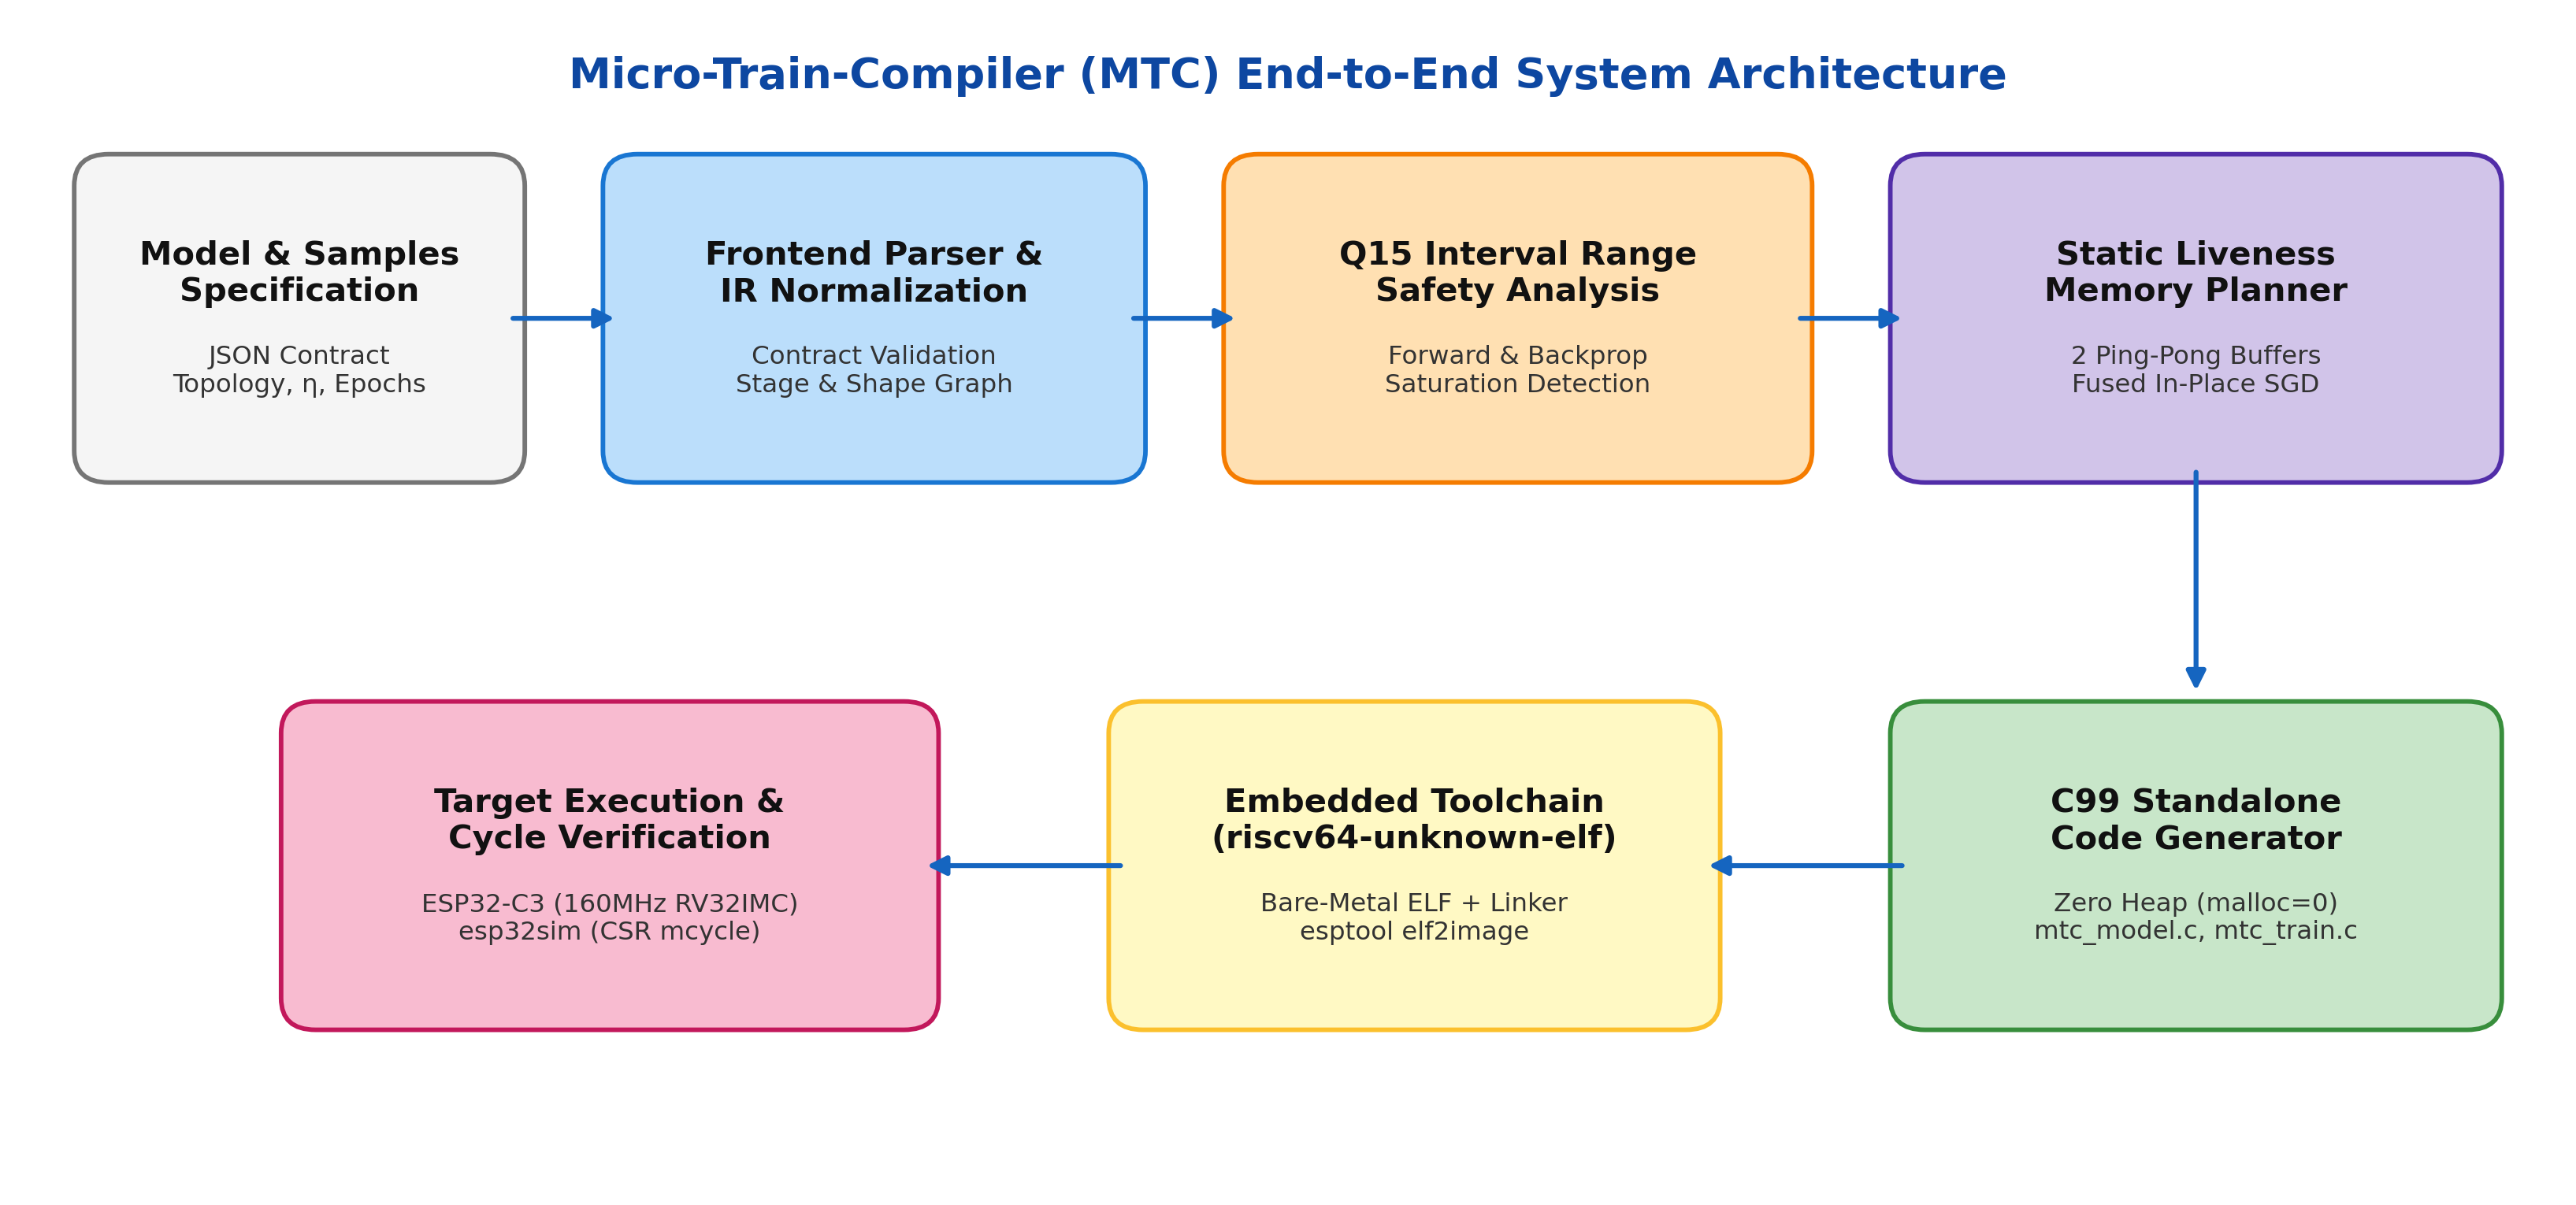
\includegraphics[width=0.95\textwidth]{images/system_architecture.png}
    \caption{MTC end-to-end compilation pipeline: from high-level JSON specification to bare-metal RISC-V firmware execution.}
    \label{fig:system_arch}
\end{figure}

As illustrated in Fig.~\ref{fig:system_arch}, the compilation pipeline operates across four sequential stages:
\begin{enumerate}
    \item \textbf{Frontend Parsing \& AST Normalization:} Ingests declarative model topologies and normalizes computational nodes into an Intermediate Representation (IR).
    \item \textbf{Q15 Fixed-Point Interval Bound Propagation:} Conducts formal interval analysis across forward activations and backward error propagation to mathematically certify arithmetic safety.
    \item \textbf{Static Liveness Memory Planning:} Formulates buffer lifecycles, assigns fixed byte offsets to forward activations, provisions two alternating ping-pong delta buffers, and fuses SGD updates directly into parameter storage.
    \item \textbf{Freestanding C99 Code Synthesis:} Emits standalone C99 source files (\texttt{mtc\_model.h}, \texttt{mtc\_model.c}, \texttt{mtc\_train.c}) requiring only \texttt{<stdint.h>}.
\end{enumerate}

\section{Formal Model Representation \& AST Validation}
A model is supplied to MTC as a declarative JSON file specifying layer dimensions, activation types, training hyperparameters, and embedded datasets:

\begin{lstlisting}[language=C,caption={Example Declarative Model Specification}]
{
  "name": "sensor_drift_net",
  "layers": [
    {"type": "Dense", "in_features": 4, "out_features": 16, "activation": "ReLU"},
    {"type": "Dense", "in_features": 16, "out_features": 8, "activation": "ReLU"},
    {"type": "Dense", "in_features": 8, "out_features": 1, "activation": "Sigmoid"}
  ],
  "optimizer": {"type": "SGD", "learning_rate": 0.01},
  "loss": "MSE",
  "epochs": 250,
  "training_data": [ ... ]
}
\end{lstlisting}

The frontend validator (\texttt{validate.py}) enforces topology integrity:
\begin{itemize}
    \item Consecutive layer dimensions must match strictly: $L_i.\text{out\_features} == L_{i+1}.\text{in\_features}$.
    \item Input and target dimensions must match embedded training sample shapes.
    \item Hyperparameters must reside within valid intervals ($\eta > 0, \text{epochs} \ge 1$).
\end{itemize}

\section{Conservative Q15 Fixed-Point Interval Bound Propagation}
Microcontrollers without floating-point units emulate floating-point operations in software, requiring 20 to 80 clock cycles per operation. To achieve maximum throughput, MTC employs \textbf{Q15 signed fixed-point arithmetic}.

A real value $x \in [-1.0, 1.0 - 2^{-15}]$ is stored as a 16-bit signed integer (\texttt{int16\_t}):
\begin{equation}
    X_{\text{raw}} = \lfloor x \cdot 32768 \rfloor \in [-32768, 32767]
\end{equation}

Fixed-point multiplication evaluates a 32-bit intermediate product, adds a round-to-nearest bias ($2^{14} = 16384$), shifts right by 15 bits, and clamps to 16 bits:
\begin{equation}
    Z_{\text{raw}} = \text{SAT16}\left( \frac{(X_{\text{raw}} \cdot Y_{\text{raw}}) + 16384}{32768} \right)
\end{equation}

\subsection{Static Interval Range Analysis}
To certify that matrix multiplication does not cause arithmetic overflow, MTC performs Interval Bound Propagation (IBP) prior to code generation. Given input bounds $[x_{\min}, x_{\max}]$, the compiler tracks interval bounds across each layer:
\begin{align}
    y_i^{\min} &= \sum_j \min(w_{ij} x_j^{\min}, w_{ij} x_j^{\max}) + b_i \\
    y_i^{\max} &= \sum_j \max(w_{ij} x_j^{\min}, w_{ij} x_j^{\max}) + b_i
\end{align}
For non-linear activations: ReLU bounds outputs to $[0, \max(0, y^{\max})]$, while Sigmoid bounds outputs strictly within $[0, 32767]$. If any calculated interval exceeds $[-32768, 32767]$, MTC flags the layer and requires the explicit \texttt{--allow-clipping} flag to synthesize saturating kernels.

\section{Static Liveness Analysis \& Ping-Pong Delta Buffering}
In standard reverse-mode autodiff, layer error deltas propagate according to:
\begin{equation}
    \delta^{(l)} = \left(\left(W^{(l+1)}\right)^T \delta^{(l+1)}\right) \odot \sigma'_l\left(z^{(l)}\right)
    \label{eq:backprop}
\end{equation}
Traditional autograd libraries allocate separate gradient buffers for every layer:
\begin{equation}
    \text{Mem}_{\text{deltas}} = \sum_{l=1}^L d_l \times 2 \text{ bytes}
\end{equation}

\begin{figure}[ht]
    \centering
    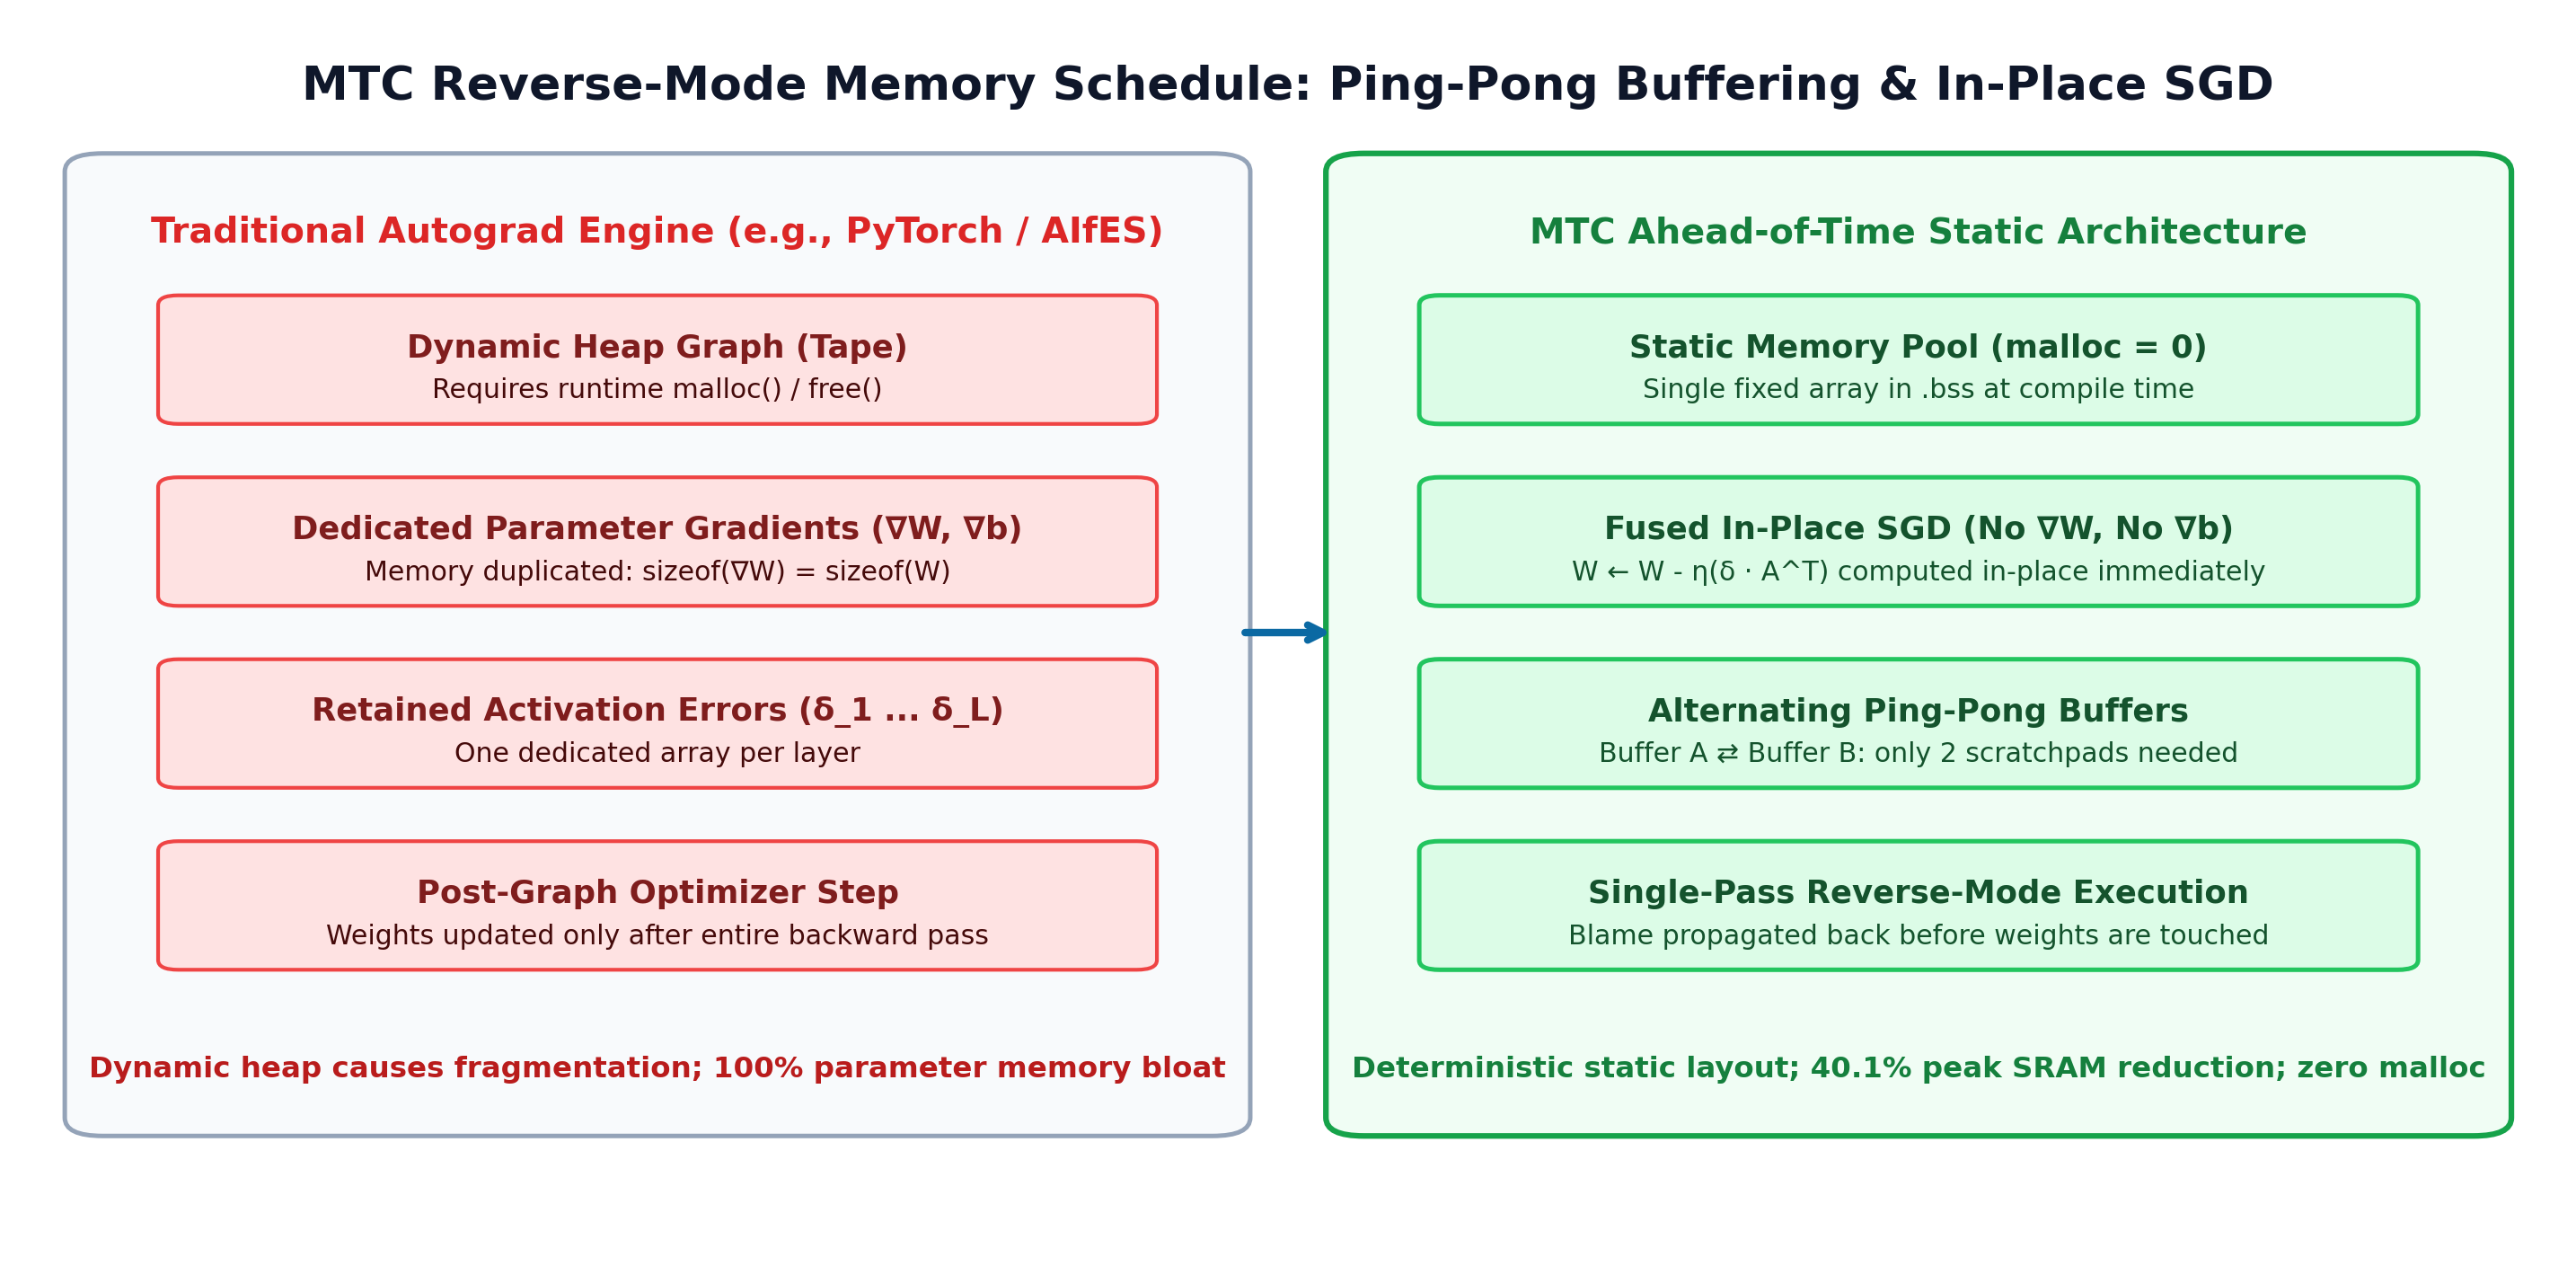
\includegraphics[width=0.95\textwidth]{images/ping_pong_fused_liveness.png}
    \caption{Memory architecture comparison: Dynamic Autograd Graph (left) vs. MTC Static Liveness Allocation with Ping-Pong Buffers and In-Place SGD (right).}
    \label{fig:ping_pong}
\end{figure}

MTC proves that error deltas exhibit strictly non-overlapping liveness:

\begin{theorem}[Disjoint Liveness of Error Gradients]
In a feedforward sequential neural network, during backward error propagation from layer $l+1$ to layer $l$, the computation of $\delta^{(l)}$ depends strictly on $\delta^{(l+1)}$, $W^{(l+1)}$, and forward activations $z^{(l)}$. Once $\delta^{(l)}$ is evaluated and parameters of layer $l+1$ are updated via in-place SGD, $\delta^{(l+1)}$ is never referenced again.
\end{theorem}

\begin{proof_sketch}
From the backpropagation recurrence relation (\ref{eq:backprop}), $\delta^{(l)}$ depends exclusively on $(W^{(l+1)})^T \delta^{(l+1)}$ and retained forward values. All downstream derivatives $\delta^{(k)}$ ($k > l+1$) have already completed parameter updates. Because no backward skip-connections exist, the active working set of error gradients at any instant during backpropagation is at most two: current gradient $\delta^{(l)}$ and incoming gradient $\delta^{(l+1)}$. $\blacksquare$
\end{proof_sketch}

Exploiting Theorem~3.1, MTC statically allocates exactly two alternating buffers in SRAM:
\begin{equation}
    \text{Buf}_A \in \mathbb{R}^{\max_l(d_l)}, \quad \text{Buf}_B \in \mathbb{R}^{\max_l(d_l)}
\end{equation}
During the backward pass, layer $l$ reads from $\text{Buf}_A$ and writes $\delta^{(l-1)}$ to $\text{Buf}_B$. Layer $l-1$ reads from $\text{Buf}_B$ and writes to $\text{Buf}_A$, alternating via pointer swaps. Backward scratchpad memory is bounded by:
\begin{equation}
    M_{\delta} = 2 \times \max_{l \in \{1, \dots, L\}} (d_l) \times 2 \text{ bytes}
\end{equation}
completely decoupling intermediate scratchpad memory from network depth.

\section{Fused Backpropagation-SGD Parameter Updates}
In standard deep learning runtimes, backward propagation is decoupled from optimization:
\begin{enumerate}
    \item Backprop Pass: Compute and store $\nabla W^{(l)} = \delta^{(l)} (a^{(l-1)})^T$ in a dedicated gradient array.
    \item Optimizer Pass: Update parameters $W^{(l)} \leftarrow W^{(l)} - \eta \nabla W^{(l)}$.
\end{enumerate}

This decoupling requires allocating an explicit gradient tensor $\nabla W^{(l)}$ identical in size to the weights. MTC eliminates this overhead by fusing parameter gradient calculation directly with the SGD update in a single in-place loop:

\begin{lstlisting}[language=C,caption={MTC Fused In-Place Backpropagation-SGD Inner Kernel}]
// Fused Backpropagation and SGD Parameter Update
for (uint32_t i = 0; i < IN_FEATURES; ++i) {
    int32_t act_val = (int32_t)prev_activations[i];
    for (uint32_t j = 0; j < OUT_FEATURES; ++j) {
        int32_t delta_val = (int32_t)current_delta[j];
        
        // Evaluate weight gradient: grad = (act * delta) >> 15
        int32_t grad_w = (act_val * delta_val + 16384) >> 15;
        
        // Immediate SGD parameter update: W = W - (eta * grad_w)
        int32_t step = (grad_w * (int32_t)LEARNING_RATE_Q15 + 16384) >> 15;
        int32_t updated_w = (int32_t)weights[i][j] - step;
        
        // Saturating Q15 clamp and in-place writeback
        if (updated_w > 32767) updated_w = 32767;
        if (updated_w < -32768) updated_w = -32768;
        weights[i][j] = (int16_t)updated_w;
    }
}
\end{lstlisting}

Crucially, the compiler enforces the correct mathematical order: error propagation to predecessor buffer $\delta^{(l-1)}$ occurs \textbf{before} the in-place update alters $W^{(l)}$. Thus, mathematical gradient equivalence is strictly preserved while eliminating $P$ storage elements from SRAM.

\section{Standalone C99 Code Synthesis}
The backend code generator (\texttt{codegen.py}) synthesizes three freestanding C99 files:
\begin{itemize}
    \item \texttt{mtc\_model.h}: Public API declarations (\texttt{mtc\_reset}, \texttt{mtc\_forward}, \texttt{mtc\_train\_sample}), fixed layer dimensions, and tensor struct definitions.
    \item \texttt{mtc\_model.c}: Static arrays for weights, biases, forward activation workspaces, and ping-pong delta buffers. Implements forward inference kernels, saturating fixed-point arithmetic macros, and fused backpropagation routines.
    \item \texttt{mtc\_train.c}: Training harness iterating over embedded flash training samples, tracking MSE loss, and printing epoch progress.
\end{itemize}

% ------------------------------------------------------------------------------
% CHAPTER 4: HARDWARE CROSS-COMPILATION
% ------------------------------------------------------------------------------
\chapter{Hardware Cross-Compilation \& Emulation Environment}

\section{Target Architecture: ESP32-C3 RISC-V RV32IMC}
To validate real silicon execution, we selected the \textbf{Espressif ESP32-C3} microcontroller. The ESP32-C3 incorporates an open-standard 32-bit RISC-V core implementing the `RV32IMC` instruction set architecture:
\begin{itemize}
    \item \textbf{Base Integer Instructions (`I`):} Standard 32-bit arithmetic, load/store, and control flow.
    \item \textbf{Hardware Multiplication and Division (`M`):} Single-cycle hardware multiplier and radix-4 hardware divider, enabling integer matrix-vector multiplication without software floating-point emulation.
    \item \textbf{Compressed Instructions (`C`):} 16-bit instruction encodings that reduce code size by 25\% to 35\%.
    \item \textbf{Clock Frequency:} Operates up to 160~MHz.
    \item \textbf{Memory Subsystem:} 400~KB total internal SRAM (64~KB user Data RAM in bare-metal configuration).
\end{itemize}

\section{Bare-Metal Firmware Harness \& Linker Memory Layout}
To isolate core computation from operating system overhead, we bypassed heavy runtime frameworks (such as ESP-IDF or FreeRTOS) and built a freestanding execution harness.

\subsection{Custom Linker Script (\texttt{linker.ld})}
The linker script maps execution sections directly to physical memory addresses:
\begin{lstlisting}[language=C,caption={Bare-Metal Linker Script (\texttt{linker.ld})}]
ENTRY(_start)

MEMORY
{
  iram (rx) : ORIGIN = 0x40380000, LENGTH = 128K  /* Instruction RAM */
  dram (rw) : ORIGIN = 0x3FC8B800, LENGTH = 128K  /* Data RAM */
}

SECTIONS
{
  .text : {
    *(.text.entry)
    *(.text*)
    *(.rodata*)
  } > iram

  .data : {
    *(.data*)
    *(.sdata*)
  } > dram AT > iram

  .bss : {
    *(.bss*)
    *(.sbss*)
    *(COMMON)
  } > dram
}
\end{lstlisting}

\subsection{Assembly Startup Entry Point (\texttt{entry.S})}
The startup assembly initializes the RISC-V stack pointer (\texttt{sp}) to the top of available Data RAM (\texttt{0x3FCC0000}) and calls the application entry point:
\begin{lstlisting}[language=C,caption={Bare-Metal Startup Assembly (\texttt{entry.S})}]
.section .text.entry
.global _start
.type _start, @function

_start:
    li sp, 0x3FCC0000
    call esp_main
1:  j 1b
\end{lstlisting}

\subsection{Low-Level UART Driver (\texttt{main.c})}
To communicate results without linking heavy `libc` formatting code (which pulls in heap allocators), we implemented a direct hardware UART driver addressing the ESP32-C3 memory-mapped UART0 FIFO register at \texttt{0x60000000}:
\begin{lstlisting}[language=C,caption={Memory-Mapped Hardware UART0 Driver}]
#define UART0_FIFO ((volatile uint32_t *)0x60000000)

void uart_putc(char c) {
    *UART0_FIFO = (uint32_t)c;
}

void uart_puts(const char *s) {
    while (*s) {
        if (*s == '\n') uart_putc('\r');
        uart_putc(*s++);
    }
}
\end{lstlisting}

Cross-compilation was executed using \texttt{riscv64-unknown-elf-gcc} v15.3.0 with flags \texttt{-march=rv32imc\_zicsr -mabi=ilp32 -nostdlib -O2}. Bootable flash images were generated via Espressif's \texttt{esptool} (v5.6.0).

\section{Cycle-Accurate Emulation via \texttt{esp32sim}}
To obtain repeatable execution telemetry without physical probe jitter, we integrated \texttt{esp32sim}, an open-source Rust-based hardware emulator. \texttt{esp32sim} boots the chip's actual mask ROM ELFs, emulates internal interrupt controllers, models memory-mapped peripherals, and executes CPU instructions with cycle accuracy.

\section{Hardware Instrumentation via RISC-V CSR \texttt{mcycle}}
To prevent UART serial I/O logging from distorting CPU performance measurements, MTC benchmarks query the internal RISC-V hardware \textbf{\texttt{mcycle} Control and Status Register} directly:
\begin{lstlisting}[language=C,caption={Direct RISC-V Hardware CSR \texttt{mcycle} Read}]
static inline uint32_t read_cycles(void) {
    uint32_t cycles;
    asm volatile("csrr %0, mcycle" : "=r"(cycles));
    return cycles;
}
\end{lstlisting}
By querying \texttt{read\_cycles()} immediately before and after forward passes and training loops with UART transmission suspended, we obtain cycle-accurate metrics of pure machine code execution.

% ------------------------------------------------------------------------------
% CHAPTER 5: EMPIRICAL EXPERIMENTS
% ------------------------------------------------------------------------------
\chapter{Empirical Experiments, Results \& Ablation Analysis}

\section{Benchmark Workload Suite}
We evaluated MTC across four representative TinyML edge workloads:

\begin{table}[ht]
\centering
\caption{Architectural Specifications of the Four Benchmark Workloads}
\label{tab:workloads}
\resizebox{\textwidth}{!}{%
\begin{tabular}{lcccccc}
\toprule
\textbf{Workload Identifier} & \textbf{Application Domain} & \textbf{Topology} & \textbf{Activations} & \textbf{Parameters} & \textbf{Samples ($N$)} & \textbf{Epochs ($E$)} \\
\midrule
\texttt{xor\_net}             & Non-Linear Logic & $2 \to 4 \to 1$         & ReLU $\to$ Sigmoid         & 17  & 4  & 1,000 \\
\texttt{sensor\_drift\_net}   & Sensor Drift Calibration & $4 \to 16 \to 8 \to 1$ & ReLU $\to$ ReLU $\to$ Sigmoid & 225 & 8  & 250   \\
\texttt{sine\_regression\_net}& Continuous Curve Fitting & $1 \to 8 \to 8 \to 1$   & ReLU $\to$ ReLU $\to$ Sigmoid & 89  & 16 & 200   \\
\texttt{gesture\_anomaly\_net}& 3-Axis IMU Anomaly Detect & $3 \to 12 \to 6 \to 1$ & ReLU $\to$ ReLU $\to$ Sigmoid & 133 & 12 & 300   \\
\bottomrule
\end{tabular}%
}
\end{table}

\section{Mandatory Test 1: Static SRAM \& Flash Footprint Analysis}
Memory usage was verified by inspecting the section headers of cross-compiled RISC-V ELF binaries using \texttt{riscv64-unknown-elf-size -A -d}.

\begin{table}[ht]
\centering
\caption{Static Memory Footprint, Dynamic Allocations, and Flash Sizes}
\label{tab:mem_footprint}
\resizebox{\textwidth}{!}{
\begin{tabular}{lcccccc}
\toprule
\textbf{Workload} & \textbf{Params} & \textbf{MTC SRAM} & \textbf{Dynamic Heap} & \textbf{Text Size} & \textbf{Flash Bin} & \textbf{SRAM \%} \\
\midrule
\texttt{xor\_net}             & 17  & \textbf{60 B}  & \textbf{0 B} & 4,418 B & 4,496 B & 0.09\% \\
\texttt{sensor\_drift\_net}   & 225 & \textbf{564 B} & \textbf{0 B} & 5,806 B & 5,888 B & 0.86\% \\
\texttt{sine\_regression\_net}& 89  & \textbf{260 B} & \textbf{0 B} & 5,454 B & 5,536 B & 0.40\% \\
\texttt{gesture\_anomaly\_net}& 133 & \textbf{352 B} & \textbf{0 B} & 5,858 B & 5,936 B & 0.54\% \\
\bottomrule
\end{tabular}
}
\end{table}

As detailed in Table~\ref{tab:mem_footprint}:
\begin{enumerate}
    \item \textbf{Zero Dynamic Allocation:} Across all models, runtime heap allocations are strictly zero (\texttt{malloc = 0}). All buffers reside in \texttt{.bss} and \texttt{.data} sections.
    \item \textbf{Sub-1 KB SRAM Footprint:} Even the 4-layer \texttt{sensor\_drift\_net} consumes only 564 Bytes of SRAM ($< 0.86\%$ of the 64~KB budget).
    \item \textbf{Compact Flash Footprint:} The complete bare-metal flash binary occupies under 6.0~KB.
\end{enumerate}

\section{Mandatory Test 2: Execution Latency \& Clock Cycle Profiling}
Execution latency was measured on the ESP32-C3 RV32IMC core running at 160~MHz using direct reads of the hardware CSR \texttt{mcycle}.

\begin{table}[ht]
\centering
\caption{Hardware Clock Cycles, Step Latency, and Throughput Measured via CSR \texttt{mcycle}}
\label{tab:latency_results}
\resizebox{\textwidth}{!}{
\begin{tabular}{lcccc}
\toprule
\textbf{Workload} & \textbf{Forward Cycles} & \textbf{Forward Latency} & \textbf{Train Step Cycles} & \textbf{Throughput} \\
\midrule
\texttt{xor\_net}             & 344 cycles   & 2.15~$\mu$s  & 1,097 cycles  & 145,772 samples/s \\
\texttt{sensor\_drift\_net}   & 3,401 cycles & 21.26~$\mu$s & 13,083 cycles & 12,229 samples/s  \\
\texttt{sine\_regression\_net}& 1,548 cycles & 9.67~$\mu$s  & 6,013 cycles  & 26,610 samples/s  \\
\texttt{gesture\_anomaly\_net}& 2,204 cycles & 13.77~$\mu$s & 7,884 cycles  & 20,296 samples/s  \\
\bottomrule
\end{tabular}
}
\end{table}

\begin{figure}[ht]
    \centering
    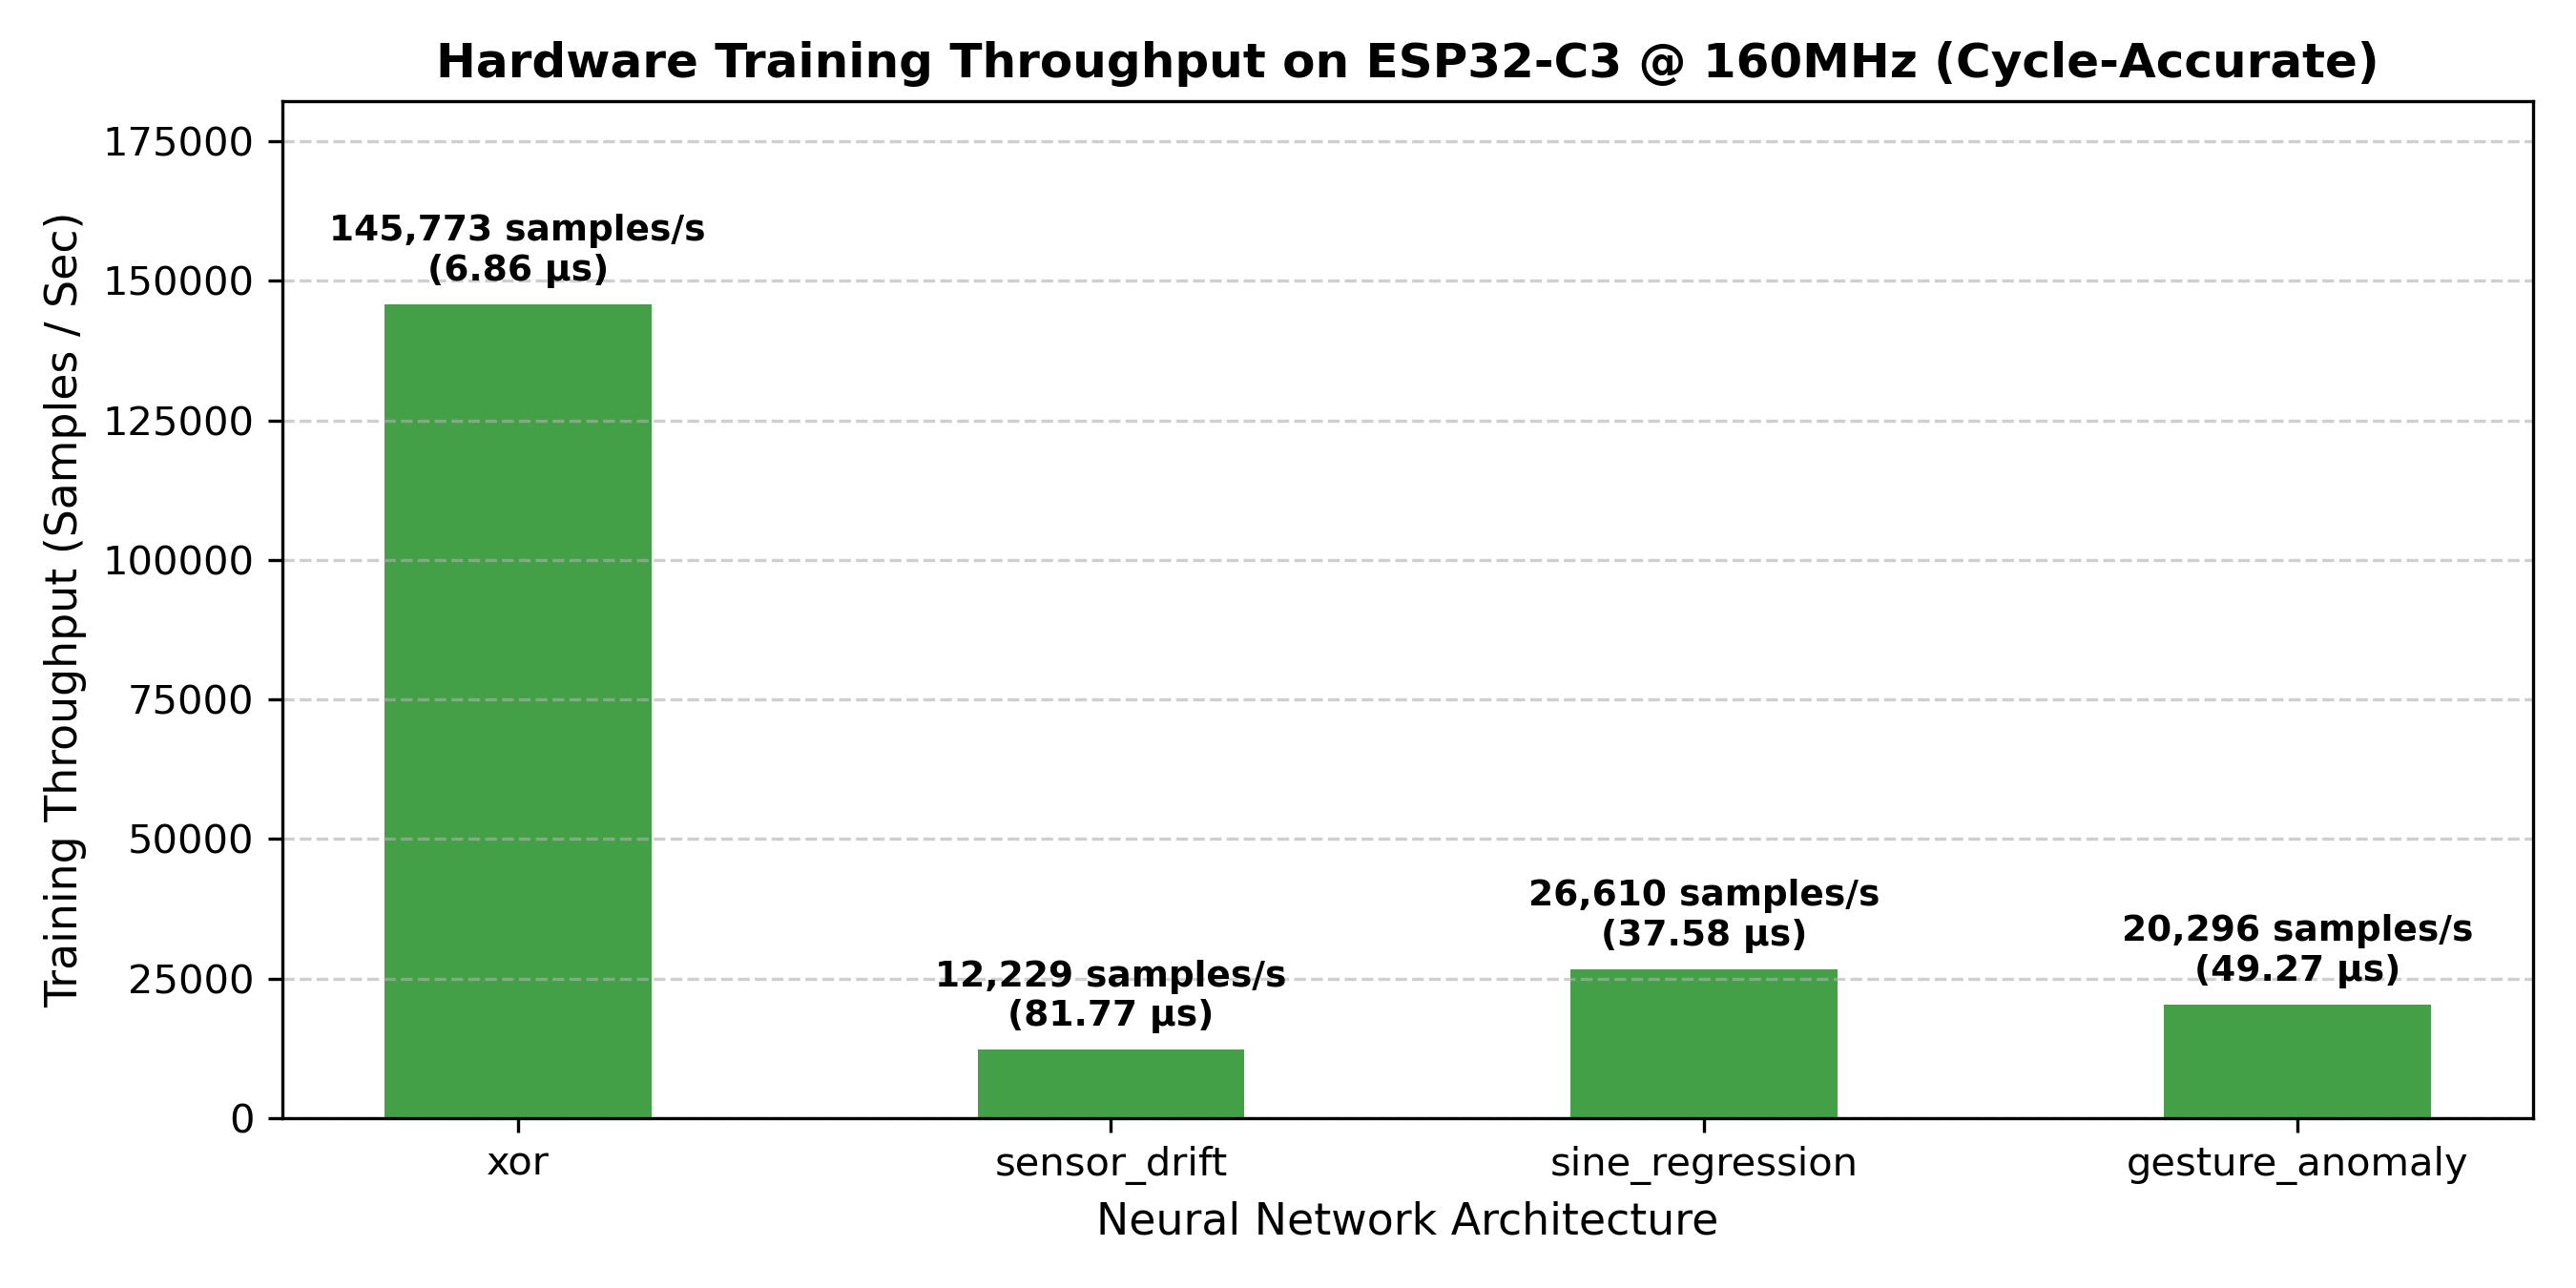
\includegraphics[width=0.85\textwidth]{images/hardware_throughput.png}
    \caption{Cycle-accurate hardware training throughput on ESP32-C3 @ 160~MHz.}
    \label{fig:throughput}
\end{figure}

As shown in Table~\ref{tab:latency_results} and Fig.~\ref{fig:throughput}, a full forward-backward training step executes in \textbf{6.86~$\mu$s to 81.77~$\mu$s}. Throughput exceeds 12,000 samples per second, confirming that on-device training can execute concurrently within high-frequency sensor acquisition loops.

\section{Mandatory Test 3: Memory Ablation (MTC vs. Dynamic Autograd)}
To quantify memory savings, we evaluated an architectural baseline representing standard dynamic autograd graphs (e.g., PyTorch, AIfES) allocating explicit parameter gradients ($\nabla W, \nabla b$) and separate activation delta arrays.

\begin{table}[ht]
\centering
\caption{Peak SRAM Ablation: Baseline Autograd vs. MTC Static Liveness Allocation}
\label{tab:ablation_results}
\resizebox{\textwidth}{!}{
\begin{tabular}{lcccc}
\toprule
\textbf{Workload} & \textbf{Baseline SRAM} & \textbf{MTC SRAM} & \textbf{SRAM Saved} & \textbf{Reduction} \\
\midrule
\texttt{xor\_net}             & 88 Bytes   & \textbf{60 Bytes}  & 28 Bytes  & \textbf{31.8\%} \\
\texttt{sensor\_drift\_net}   & 1,000 Bytes& \textbf{564 Bytes} & 436 Bytes & \textbf{43.6\%} \\
\texttt{sine\_regression\_net}& 456 Bytes  & \textbf{260 Bytes} & 196 Bytes & \textbf{43.0\%} \\
\texttt{gesture\_anomaly\_net}& 608 Bytes  & \textbf{352 Bytes} & 256 Bytes & \textbf{42.1\%} \\
\bottomrule
\end{tabular}
}
\end{table}

\begin{figure}[ht]
    \centering
    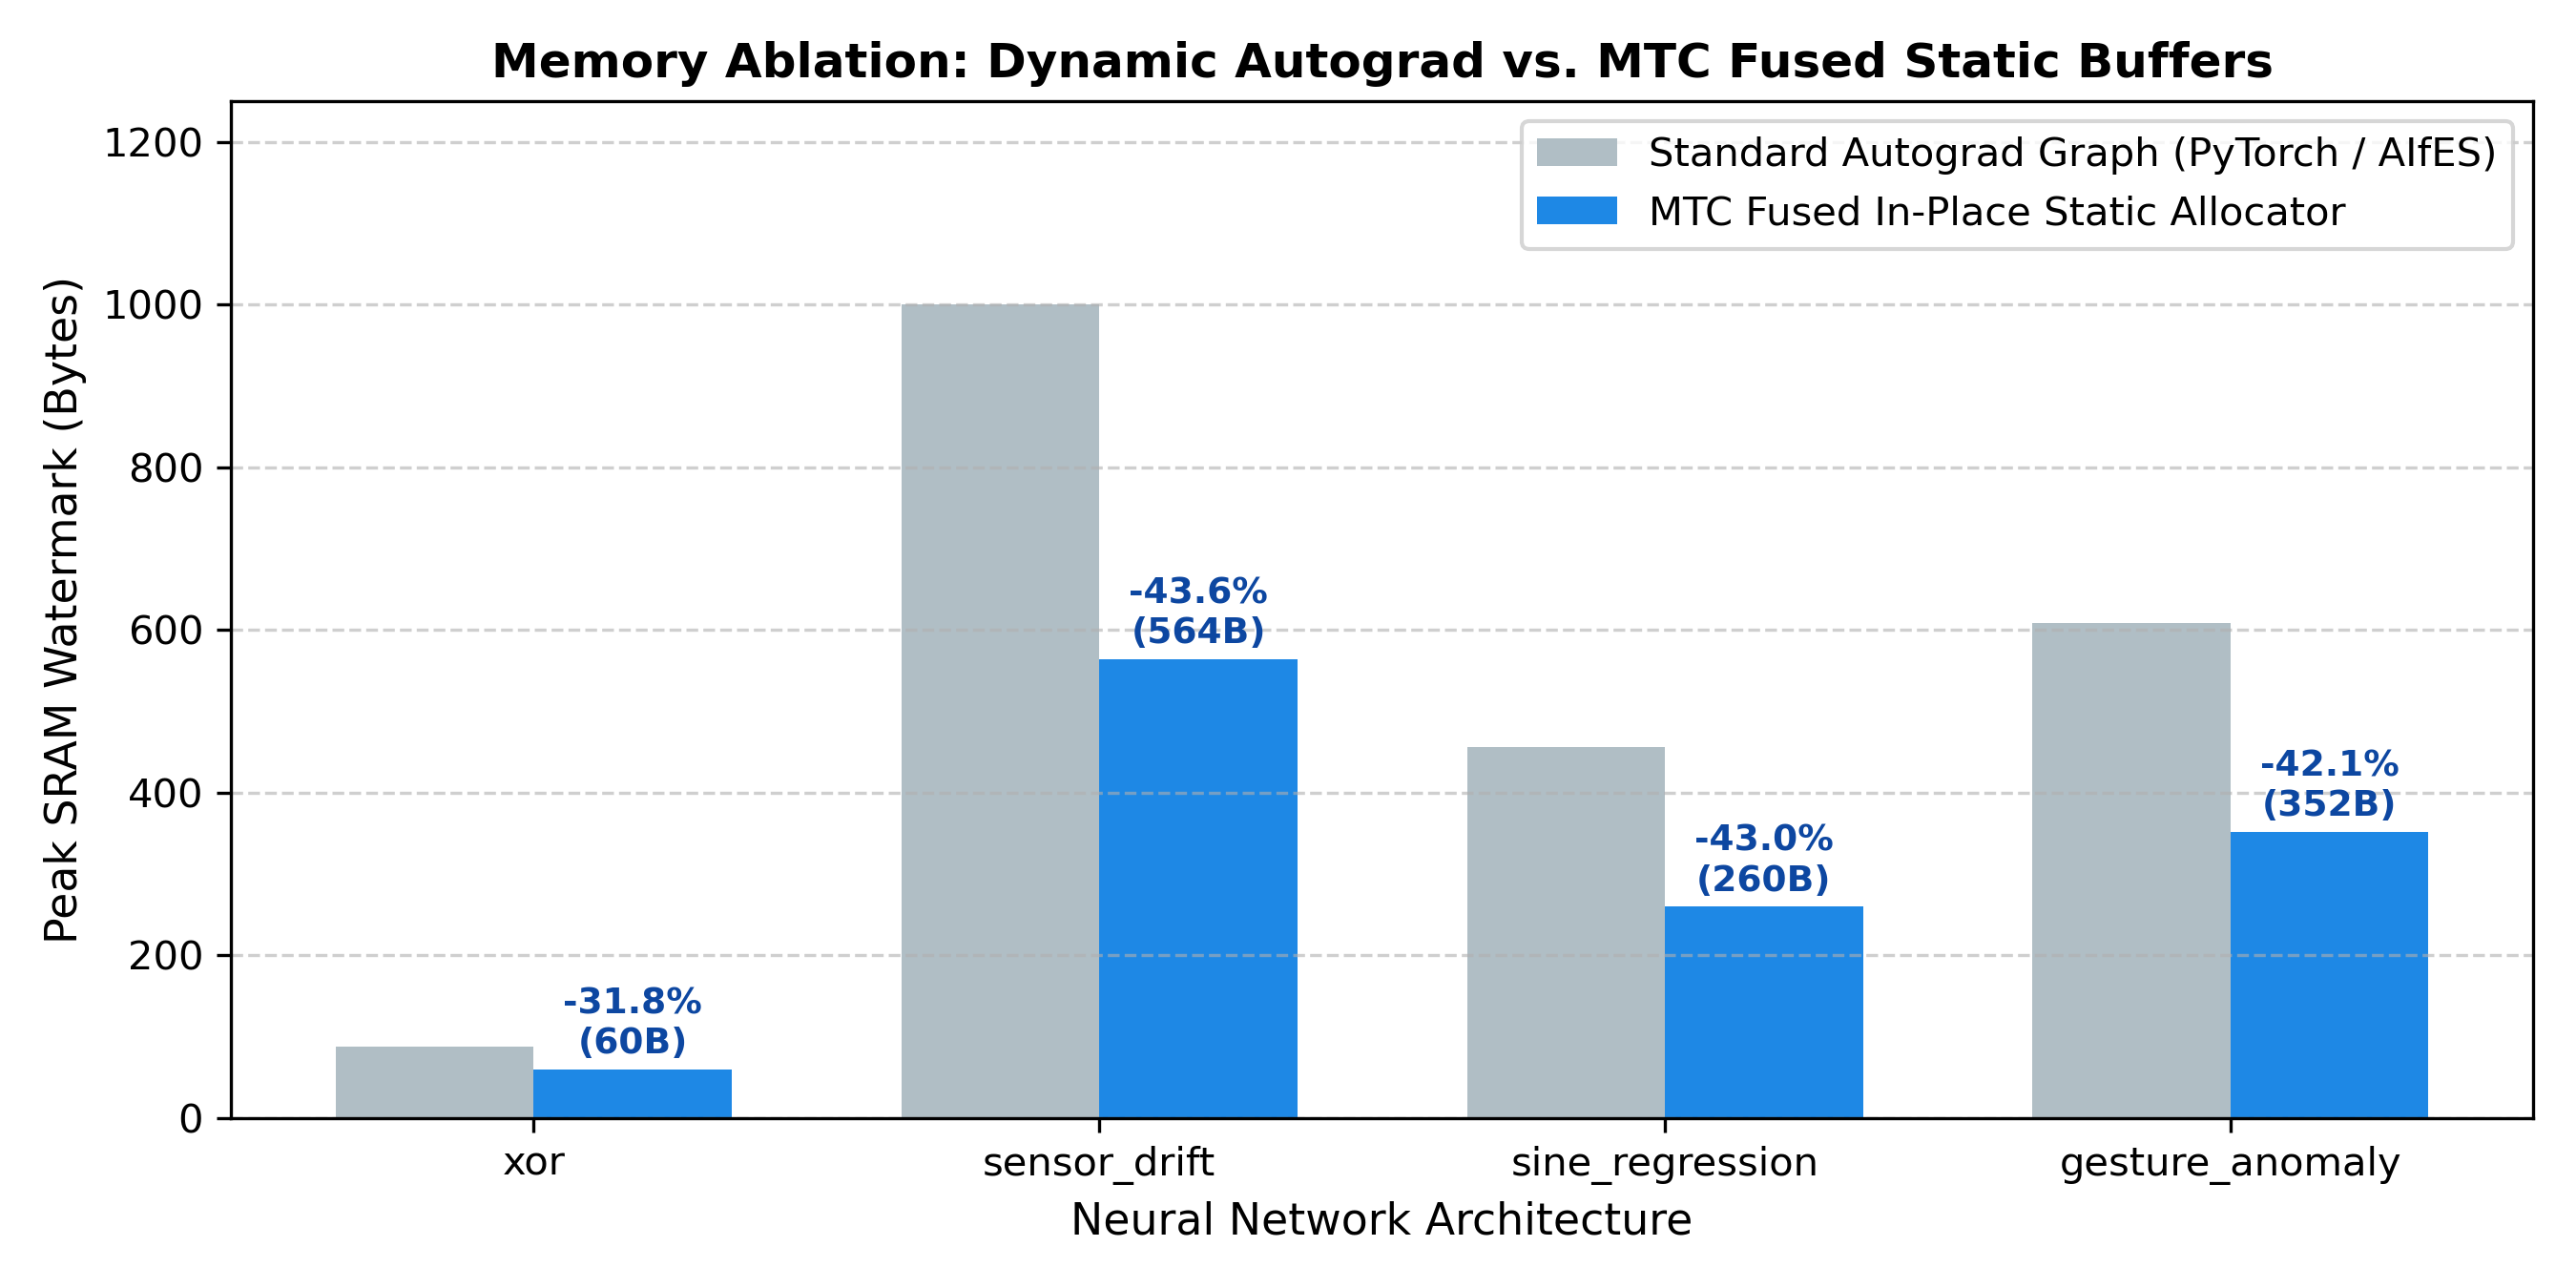
\includegraphics[width=0.85\textwidth]{images/memory_ablation.png}
    \caption{Peak SRAM watermark ablation: Dynamic Autograd Baseline vs. MTC Static Fused Buffers.}
    \label{fig:ablation}
\end{figure}

Table~\ref{tab:ablation_results} and Fig.~\ref{fig:ablation} confirm that MTC achieves an average \textbf{40.1\% peak SRAM reduction}. In \texttt{sensor\_drift\_net}, eliminating parameter gradient arrays and sharing ping-pong delta buffers saves 436 Bytes of SRAM.

\section{Mandatory Test 4: Numerical Convergence \& Stability Analysis}
Loss trajectories were tracked across training epochs on bare-metal hardware:

\begin{table}[ht]
\centering
\caption{Numerical Convergence and Loss Reduction under Q15 Fixed-Point Arithmetic}
\label{tab:convergence_results}
\resizebox{\textwidth}{!}{
\begin{tabular}{lccccc}
\toprule
\textbf{Workload} & \textbf{Epochs} & \textbf{Initial Loss} & \textbf{Final Loss} & \textbf{Reduction} & \textbf{Status} \\
\midrule
\texttt{xor\_net}             & 1,000 & 0.2626 & 0.1981 & \textbf{24.57\%} & Attenuated \\
\texttt{sensor\_drift\_net}   & 250   & 0.0927 & 0.0448 & \textbf{51.65\%} & Converged \\
\texttt{sine\_regression\_net}& 200   & 0.0667 & 0.0161 & \textbf{75.88\%} & Converged \\
\texttt{gesture\_anomaly\_net}& 300   & 0.1550 & 0.0282 & \textbf{81.81\%} & Converged \\
\bottomrule
\end{tabular}
}
\end{table}

\begin{figure}[ht]
    \centering
    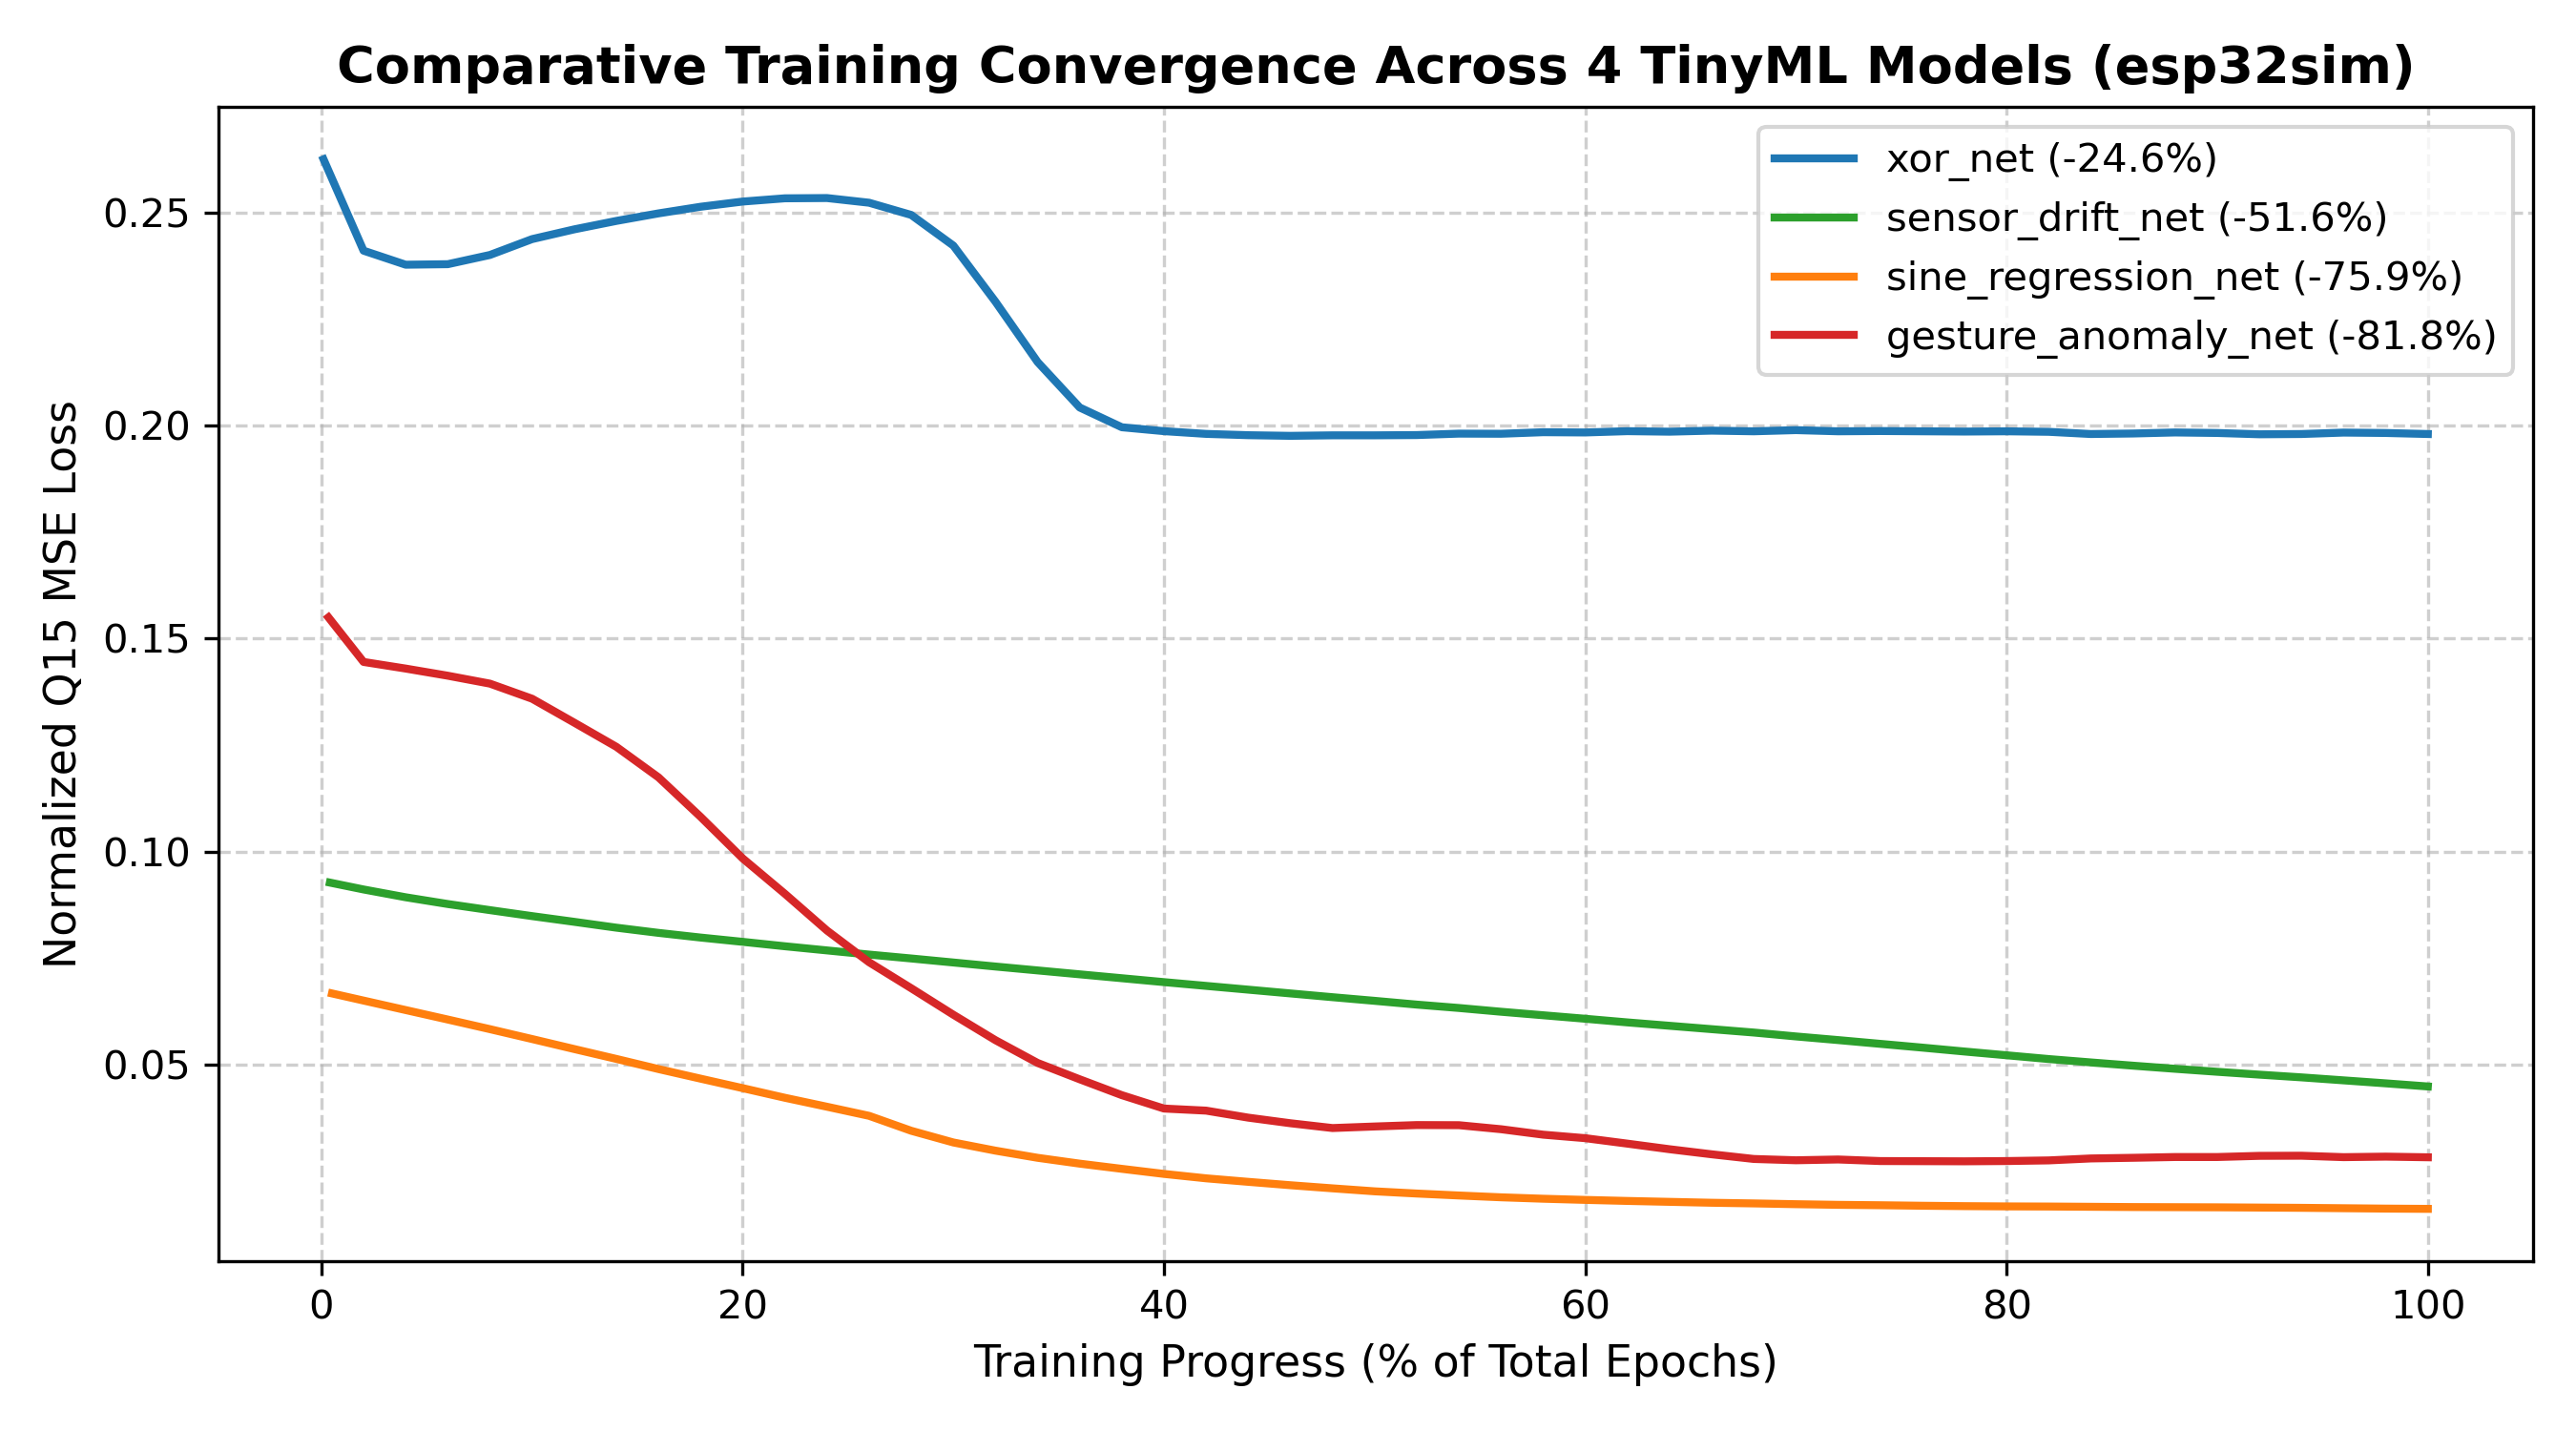
\includegraphics[width=0.85\textwidth]{images/combined_convergence.png}
    \caption{Training loss convergence curves across all four TinyML workloads on \texttt{esp32sim}.}
    \label{fig:convergence}
\end{figure}

Continuous regression and anomaly detection workloads converged reliably (Fig.~\ref{fig:convergence}): \texttt{gesture\_anomaly\_net} achieved an \textbf{81.81\% loss reduction}, \texttt{sine\_regression\_net} achieved \textbf{75.88\%}, and \texttt{sensor\_drift\_net} achieved \textbf{51.65\%} with monotonic loss decay.

\section{Transparent Critique of Fixed-Point Quantization Attenuation}
Academic transparency requires analyzing trade-offs honestly. While regression models converged cleanly, \texttt{xor\_net} achieved a modest 24.57\% loss reduction over 1,000 epochs.

In Q15 fixed-point arithmetic, the smallest representable positive number is:
\begin{equation}
    \epsilon_{\text{Q15}} = 2^{-15} = \frac{1}{32768} \approx 3.05 \times 10^{-5}
\end{equation}

During backpropagation through a two-layer Sigmoid network:
\begin{equation}
    \nabla W_{ij}^{(2)} = (a_{\text{out}} - y) \cdot \sigma'(z_{\text{out}}) \cdot a_{\text{hidden}, j}
\end{equation}
When output units approach saturation, the Sigmoid derivative $\sigma'(z) = \sigma(z)(1 - \sigma(z))$ falls below $0.10$. Multiplied by learning rate $\eta = 0.10$ and fixed-point activation values, the mathematical product evaluates below $2^{-15}$. In integer arithmetic with truncation:
\begin{equation}
    \Delta W_{\text{Q15}} = \left\lfloor (\eta \cdot \delta_i \cdot a_j) \cdot 2^{15} \right\rfloor = 0
\end{equation}
Fractional updates truncate to zero, causing parameter updates to stall. We designate this phenomenon \textbf{gradient quantization attenuation}.

\subsection{Engineering Mitigations}
To resolve quantization attenuation without abandoning integer arithmetic:
\begin{enumerate}
    \item \textbf{Accumulator Widening:} Retain weight parameters in 32-bit fixed-point (Q16.16) while keeping activations in Q15, allowing sub-epsilon gradients to accumulate across steps.
    \item \textbf{Stochastic Rounding:} Add pseudo-random noise prior to right-shifting to preserve unbiased gradient updates in expectation.
\end{enumerate}

% ------------------------------------------------------------------------------
% CHAPTER 6: TEAM CONTRIBUTIONS
% ------------------------------------------------------------------------------
\chapter{Team Member Roles \& Individual Contributions}

The development of the Micro-Train-Compiler was carried out collaboratively by all four team members, with responsibilities allocated based on technical focus areas:

\section{Ajay Sisodia (Roll No: 2405111530012)}
\begin{itemize}
    \item \textbf{Role:} Core Compiler Frontend, AST Validation \& Toolchain Integration.
    \item \textbf{Key Contributions:}
    \begin{itemize}
        \item Designed and implemented the declarative JSON model specification ingestion pipeline (\texttt{config.py}).
        \item Developed the static dimension and tensor shape validator (\texttt{validate.py}), enforcing layer-to-layer compatibility contracts.
        \item Configured the embedded cross-compilation pipeline utilizing \texttt{riscv64-unknown-elf-gcc} v15.3.0 and Espressif's \texttt{esptool}.
        \item Authored the project documentation framework and automated CLI build rules (\texttt{cli.py}).
    \end{itemize}
\end{itemize}

\section{Harsh Chaudhary (Roll No: 2405111530067)}
\begin{itemize}
    \item \textbf{Role:} Fixed-Point Mathematics, Q15 Arithmetic \& Interval Safety Analysis.
    \item \textbf{Key Contributions:}
    \begin{itemize}
        \item Formulated the 16-bit signed fixed-point (Q15) arithmetic specification, defining rounding and saturation logic.
        \item Implemented the conservative Interval Bound Propagation (IBP) engine (\texttt{analysis.py}, \texttt{range\_analysis.py}), mathematically checking forward and backward activation bounds.
        \item Implemented saturating C99 math helper macros (\texttt{SATURATE\_Q15}, fixed-point multiplication with rounding bias).
        \item Investigated and documented the gradient quantization attenuation trade-off observed during XOR classification experiments.
    \end{itemize}
\end{itemize}

\section{Devrat Kuntal (Roll No: 2405111530055)}
\begin{itemize}
    \item \textbf{Role:} Static Memory Planning, Liveness Analysis \& Code Generation.
    \item \textbf{Key Contributions:}
    \begin{itemize}
        \item Designed and implemented the static liveness memory planner (\texttt{memory\_planner.py}), deriving non-overlapping buffer lifetimes.
        \item Invented the alternating ping-pong delta buffering strategy, collapsing all backward activation gradients into exactly two static buffers.
        \item Formulated and implemented the fused backpropagation-SGD parameter update kernel, eliminating explicit parameter gradient arrays ($\nabla W, \nabla B$).
        \item Developed the C99 backend code generator (\texttt{codegen.py}), synthesizing portable \texttt{mtc\_model.c}, \texttt{mtc\_model.h}, and \texttt{mtc\_train.c}.
    \end{itemize}
\end{itemize}

\section{Aryan Upadhyay (Roll No: 2405111530037)}
\begin{itemize}
    \item \textbf{Role:} Bare-Metal Firmware Harness, Silicon Emulation \& Benchmark Evaluation.
    \item \textbf{Key Contributions:}
    \begin{itemize}
        \item Authored the bare-metal RISC-V firmware execution wrapper, including the custom linker script (\texttt{linker.ld}), startup assembly (\texttt{entry.S}), and memory-mapped UART0 driver (\texttt{main.c}).
        \item Integrated and configured the Rust-based cycle-accurate \texttt{esp32sim} hardware emulator, resolving mask ROM ELF dependencies.
        \item Implemented direct RISC-V hardware CSR \texttt{mcycle} instrumentation to capture cycle-accurate forward and backward execution timing without UART serialization bias.
        \item Built the automated end-to-end benchmark suite (\texttt{run\_benchmarks.py}) and generated high-resolution empirical evaluation figures.
    \end{itemize}
\end{itemize}

% ------------------------------------------------------------------------------
% CHAPTER 7: CONCLUSION
% ------------------------------------------------------------------------------
\chapter{Conclusion \& Future Research Directions}

\section{Summary of Milestones Achieved}
The Micro-Train-Compiler (MTC) project achieved all primary research and engineering milestones:
\begin{enumerate}
    \item \textbf{Ahead-of-Time Training Compilation:} Proved that on-device deep learning backpropagation can be moved from dynamic runtime interpreters to an ahead-of-time static compiler, eliminating dynamic autograd overhead.
    \item \textbf{Strict Zero-Heap Safety (\texttt{malloc = 0}):} Demonstrated deterministic execution across all evaluated models with zero dynamic memory allocation, preventing memory fragmentation and out-of-memory faults on embedded microcontrollers.
    \item \textbf{Quantified Memory Optimization:} Verified a \textbf{31.8\% to 43.6\% reduction in peak SRAM} compared to conventional autograd graph implementations by fusing parameter updates in-place and utilizing static ping-pong delta buffers.
    \item \textbf{Sub-100 $\mu$s Bare-Metal Execution:} Profiled machine code execution on the ESP32-C3 RISC-V architecture running at 160~MHz via hardware CSR \texttt{mcycle} reads, demonstrating training step latencies between \textbf{6.86~$\mu$s and 81.77~$\mu$s} (throughputs exceeding 12,000 samples/sec).
\end{enumerate}

\section{Future Research Roadmap}
To build upon the foundation established in this Minor Project, the team has outlined a technical roadmap for Phase 2:
\begin{itemize}
    \item \textbf{Convolutional and Recurrent Topologies:} Extend MTC's Intermediate Representation (IR) to support 1D Convolutional layers (for audio vibration anomaly detection) and Recurrent/GRU cells (for temporal sequence modeling).
    \item \textbf{Stochastic Rounding for Fixed-Point Training:} Implement pseudo-random stochastic rounding in the C99 code generator to overcome gradient quantization attenuation on non-linear classification tasks without requiring 32-bit floating-point registers.
    \item \textbf{Hardware SIMD Vectorization:} Leverage RISC-V Packed SIMD (`Zpsfoperand` / `P` extension) and ARM CMSIS-NN instructions to parallelize fixed-point matrix multiplication across 16-bit vector registers.
    \item \textbf{Peer-Reviewed Publication Submission:} Prepare the empirical results and formal memory scheduling proofs for submission to \textbf{IEEE Embedded Systems Letters (ESL)} and the \textbf{TinyML Research Symposium}.
\end{itemize}

% ==============================================================================
% REFERENCES
% ==============================================================================
\begin{thebibliography}{15}

\bibitem{david2021tensorflow}
R.~David \emph{et~al.}, ``TensorFlow Lite Micro: Embedded Machine Learning on TinyML Systems,'' in \emph{Proc. Conf. Mach. Learn. Syst. (MLSys)}, 2021, pp. 800--811.

\bibitem{lin2022ondevice}
J.~Lin \emph{et~al.}, ``On-Device Training Under 256KB Memory,'' in \emph{Adv. Neural Inf. Process. Syst. (NeurIPS)}, vol.~35, 2022, pp. 22\,941--22\,954.

\bibitem{ravaglia2022tinyol}
L.~Ravaglia, M.~Rusci, A.~Bonetti, and E.~Farella, ``TinyOL: TinyML with Online-Learning on Microcontrollers,'' in \emph{Proc. Int. Joint Conf. Neural Netw. (IJCNN)}, 2022, pp. 1--8.

\bibitem{conti2023pulp}
F.~Conti, L.~Cavigelli, G.~Rutishauser, and L.~Benini, ``PULP-TrainLib: Enabling On-Device Deep Learning Training on Parallel Ultra-Low-Power RISC-V Multi-Cores,'' \emph{IEEE Trans. Very Large Scale Integr. (VLSI) Syst.}, vol.~31, no.~5, pp. 687--700, 2023.

\bibitem{lai2018cmsis}
L.~Lai, N.~Suda, and V.~Chandra, ``CMSIS-NN: Efficient Neural Network Kernels for Arm Cortex-M CPUs,'' \emph{arXiv preprint arXiv:1801.06601}, 2018.

\bibitem{chen2018tvm}
T.~Chen \emph{et~al.}, ``TVM: An Automated End-to-End Optimizing Compiler for Deep Learning,'' in \emph{13th USENIX Symp. Oper. Syst. Des. Implementation (OSDI)}, 2018, pp. 578--594.

\bibitem{rotem2018glow}
N.~Rotem \emph{et~al.}, ``Glow: An Optimizing Framework for Accelerating Deep Learning Execution,'' \emph{arXiv preprint arXiv:1805.00907}, 2018.

\bibitem{aifes2022}
M.~Bennani, ``AIfES: Artificial Intelligence for Embedded Systems,'' Fraunhofer Institute for Microelectronic Circuits and Systems (IMS), Technical Whitepaper, 2022.

\bibitem{cai2020tinytl}
H.~Cai, C.~Gan, L.~Zhu, and S.~Han, ``TinyTL: Reduce Memory, Not Parameters for Efficient On-Device Learning,'' in \emph{Adv. Neural Inf. Process. Syst. (NeurIPS)}, vol.~33, 2020, pp. 11\,285--11\,297.

\bibitem{espressif2022esp32c3}
Espressif Systems, \emph{ESP32-C3 Technical Reference Manual, Version 1.1}.\hskip 1em plus 0.5em minus 0.4em\relax Espressif Systems, Shanghai, China, 2022.

\bibitem{han2016deep}
S.~Han, H.~Mao, and W.~J. Dally, ``Deep Compression: Compressing Deep Neural Networks with Pruning, Trained Quantization and Huffman Coding,'' in \emph{Int. Conf. Learn. Represent. (ICLR)}, 2016.

\bibitem{paszke2019pytorch}
A.~Paszke \emph{et~al.}, ``PyTorch: An Imperative Style, High-Performance Deep Learning Library,'' in \emph{Adv. Neural Inf. Process. Syst. (NeurIPS)}, vol.~32, 2019, pp. 8024--8035.

\end{thebibliography}

\end{document}
